%\SweaveOpts{prefix.string=prova3e,
%\SweaveOpts{prefix.string=figs/av01,width=6,height=6,eps=TRUE}

\documentclass[11pt,a4]{article}\usepackage[]{graphicx}\usepackage[]{xcolor}
% maxwidth is the original width if it is less than linewidth
% otherwise use linewidth (to make sure the graphics do not exceed the margin)
\makeatletter
\def\maxwidth{ %
  \ifdim\Gin@nat@width>\linewidth
    \linewidth
  \else
    \Gin@nat@width
  \fi
}
\makeatother

\definecolor{fgcolor}{rgb}{0.345, 0.345, 0.345}
\newcommand{\hlnum}[1]{\textcolor[rgb]{0.686,0.059,0.569}{#1}}%
\newcommand{\hlsng}[1]{\textcolor[rgb]{0.192,0.494,0.8}{#1}}%
\newcommand{\hlcom}[1]{\textcolor[rgb]{0.678,0.584,0.686}{\textit{#1}}}%
\newcommand{\hlopt}[1]{\textcolor[rgb]{0,0,0}{#1}}%
\newcommand{\hldef}[1]{\textcolor[rgb]{0.345,0.345,0.345}{#1}}%
\newcommand{\hlkwa}[1]{\textcolor[rgb]{0.161,0.373,0.58}{\textbf{#1}}}%
\newcommand{\hlkwb}[1]{\textcolor[rgb]{0.69,0.353,0.396}{#1}}%
\newcommand{\hlkwc}[1]{\textcolor[rgb]{0.333,0.667,0.333}{#1}}%
\newcommand{\hlkwd}[1]{\textcolor[rgb]{0.737,0.353,0.396}{\textbf{#1}}}%
\let\hlipl\hlkwb

\usepackage{framed}
\makeatletter
\newenvironment{kframe}{%
 \def\at@end@of@kframe{}%
 \ifinner\ifhmode%
  \def\at@end@of@kframe{\end{minipage}}%
  \begin{minipage}{\columnwidth}%
 \fi\fi%
 \def\FrameCommand##1{\hskip\@totalleftmargin \hskip-\fboxsep
 \colorbox{shadecolor}{##1}\hskip-\fboxsep
     % There is no \\@totalrightmargin, so:
     \hskip-\linewidth \hskip-\@totalleftmargin \hskip\columnwidth}%
 \MakeFramed {\advance\hsize-\width
   \@totalleftmargin\z@ \linewidth\hsize
   \@setminipage}}%
 {\par\unskip\endMakeFramed%
 \at@end@of@kframe}
\makeatother

\definecolor{shadecolor}{rgb}{.97, .97, .97}
\definecolor{messagecolor}{rgb}{0, 0, 0}
\definecolor{warningcolor}{rgb}{1, 0, 1}
\definecolor{errorcolor}{rgb}{1, 0, 0}
\newenvironment{knitrout}{}{} % an empty environment to be redefined in TeX

\usepackage{alltt}
\usepackage[utf8]{inputenc}
\usepackage[brazil,brazilian]{babel}
\usepackage[top=0.5cm,left=0.7cm,bottom=0.5cm,right=1.2cm,nohead]{geometry}
\usepackage{amssymb}   % símbolos matemáticos extras
\usepackage{amsmath}
\usepackage{amsbsy}   % símbolos matemáticos em negrito
\usepackage{graphicx}
\usepackage{comment}
\usepackage{array}
\usepackage{multirow}

\excludecomment{solucao}
%\includecomment{solucao}
\renewcommand\ThisComment[1]{%
  \immediate\write\CommentStream{\unexpanded{#1}}%
}
%\excludecomment{extra}
\includecomment{extra}

%\usepackage{Sweave}
\title{Inferência Bayesiana}
\author{}
% \author{\textbf{GRR: }  \raisebox{-0.5ex}{\rule{1.4in}{0.01in}} \textbf{Nome: } \raisebox{-0.5ex}{\rule{3.8in}{0.01in}} }
\date{}



\IfFileExists{upquote.sty}{\usepackage{upquote}}{}
\begin{document}
\maketitle

%\vspace{-0.5in}
\pagestyle{empty}
\thispagestyle{empty}

\sloppy

\begin{enumerate}

%%%
%%% $1^a$ Prova (17/10/2025)
%%%
\item Modela-se com a distribuição binomial negativa o número de entrevistas necessárias para se conseguir três candidatos aprovados em uma fase inicial de um processo seletivo. Considera-se uma abordagem Bayesiana. Não se tem ideia da probabilidade de aprovação e decide-se por uma distribuição {\it a priori} que reflita tal situação. Em uma rodada de seleção foram necessárias 20 entrevistas para se conseguir os três aprovados. 
  \begin{enumerate}
  \item Escreva a função de densidade de probabilidades para a probabilidade de aprovação antes da rodada de seleção.
  \item Escreva a função de verossimilhança. 
  \item Reconheça uma distribuição de probabilidades proporcional à esta expressão da verossimilhança. Qual é a distribuição e com quais valores de parâmetros? 
  \item Forneça a expressão de uma distribuição à {\it priori} conjugada que poderia ser utilizada caso houvesse alguma suspeita sobre valores não uniformes para a probabilidade de aprovação.
  \item Qual(ais) valor(es) você especificaria para o(s) parâmetro(s) da distribuição {\it priori} conjugada (hiperparâmetros) neste caso? Justifique.
  \item Como é obtida a distribuição marginal (preditiva a priori)?
  \item Explique como faria para simular valores desta distribuição marginal.
  \item Obtenha a expressão da posteriori e indique qual a distribuição de probabilidades.
  \item Qual(ais) quantidade(s) calculada(s) com a amostra são necessárias para a obtenção da verossimilhança e posteriori?
  \item Forneça a expressão da distribuição a posteriori para $\theta$ com os dados da rodada de seleção.
  \item Qual o valor esperado da distribuição a posteriori para $\theta$?
%  \item Mostre que o valor esperado da posteriori é uma média ponderada entre o valor esperado da priori e do estimador de máxima verossimilhança. 
  \item Como poderia ser obtida a distribuição preditiva para uma nova observação após obter esta primeira amostra?
  \item Como obter o valor esperado da preditiva do item anterior?
  \item Foi necessário fazer uma segunda rodada de seleção na qual foram necessárias 15 entrevistas para se conseguir os 3 aprovados. Qual a posteriori após também considerar os dados desta segunda rodada de seleção? 
  \end{enumerate}

\item Dentre usuários que se cadastram em uma plataforma, 20\% declaram ter menos de 25 anos e acredita-se que destes, 10\% utiliza perfil falso. Entre 25 e 50 anos são 50\% dos usuários, com 20\% deles sendo perfis falsos. Acima de 50 anos são 30\% dos usuários e 5\% deles com perfis falso. Toma-se um usuário ao acaso e verifica-se que possui perfil falso.
\begin{enumerate}
\item Sem fazer contas, qual faixa etária que voce espera ser a deste usuário? Justifique.
\item Qual a probabilidade de ser de cada uma das faixas etárias? Resolva a problema da forma que achar adequada.
\item Considere agora o problema do ponto de vista Bayesiano.
\begin{itemize}
\item Qual é a variável resposta $(Y)$ e sua distribuição?0
\item Qual é o parâmetro $(\theta)$ e sua distribuição a {\it priori}?
\item Qual a verossimilhança? E a {\it posteriori}? E a marginal (preditiva)?
\end{itemize}
\item Esboce um gráfico da {\it priori} e da {\it posteriori}.
\item Interprete os resultados.
\item Agora que resolveu o problema, a qual faixa etária voce espera o usuário pertencer? Justifique.
\item As proporções de perfis masculinos são de 15\%, 30\% e 55\% para as faixas etárias de menos de 25 anos, entre 25 e 50 anos e acima de 50 anos, respectivamente. Se o usuário de perfil falso selecionado for do sexo masculino, qual a probabilidade de pertencer a cada uma das faixas etárias?
\end{enumerate}

\newpage

\item Indique para cada trecho de código a seguir o modelo usado e o que está sendo obtido.
  
\begin{enumerate}

\item
\begin{knitrout}
\definecolor{shadecolor}{rgb}{0.969, 0.969, 0.969}\color{fgcolor}\begin{kframe}
\begin{alltt}
\hldef{vec1} \hlkwb{<-} \hlkwd{runif}\hldef{(}\hlnum{1E5}\hldef{)}
\hldef{vec2} \hlkwb{<-} \hlkwd{rbinom}\hldef{(}\hlnum{1E5}\hldef{,} \hlkwc{size} \hldef{=} \hlnum{20}\hldef{,} \hlkwc{prob} \hldef{= vec1)}
\hlkwd{plot}\hldef{(}\hlkwd{table}\hldef{(}\hlkwd{factor}\hldef{(vec2,} \hlkwc{levels} \hldef{=} \hlnum{0}\hlopt{:}\hlnum{20}\hldef{)),} \hlkwc{type} \hldef{=} \hlsng{'h'}\hldef{)}
\hlkwd{mean}\hldef{(vec2} \hlopt{>} \hlnum{5}\hldef{)}
\hldef{vec3} \hlkwb{<-} \hlkwd{rbeta}\hldef{(}\hlnum{1E5}\hldef{,} \hlnum{8}\hlopt{+}\hlnum{1}\hldef{, (}\hlnum{20}\hlopt{-}\hlnum{8}\hldef{)}\hlopt{+}\hlnum{1}\hldef{)}
\hlkwd{hist}\hldef{(vec3,} \hlkwc{freq} \hldef{=} \hlnum{FALSE}\hldef{,} \hlkwc{nclass} \hldef{=} \hlnum{30}\hldef{)}
\hlkwd{mean}\hldef{(vec3} \hlopt{<} \hlnum{0.30}\hldef{)}
\end{alltt}
\end{kframe}
\end{knitrout}

\item
\begin{knitrout}
\definecolor{shadecolor}{rgb}{0.969, 0.969, 0.969}\color{fgcolor}\begin{kframe}
\begin{alltt}
\hlkwd{curve}\hldef{(}\hlkwd{dbeta}\hldef{(x,} \hlnum{2}\hldef{,} \hlnum{8}\hldef{),} \hlkwc{ylim} \hldef{=} \hlkwd{c}\hldef{(}\hlnum{0}\hldef{,} \hlnum{7}\hldef{))}
\hlkwd{curve}\hldef{(}\hlkwd{dbeta}\hldef{(x,} \hlnum{2} \hlopt{+} \hlnum{10}\hldef{,} \hlnum{8} \hlopt{+} \hlnum{30}\hldef{),} \hlkwc{col} \hldef{=} \hlnum{4}\hldef{,} \hlkwc{add} \hldef{=} \hlnum{TRUE}\hldef{)}
\hldef{vec1} \hlkwb{<-} \hlkwd{rbeta}\hldef{(}\hlnum{1E5}\hldef{,} \hlnum{2} \hlopt{+} \hlnum{10}\hldef{,} \hlnum{8} \hlopt{+} \hlnum{30}\hldef{)}
\hldef{vec2} \hlkwb{<-} \hlkwd{rbinom}\hldef{(}\hlnum{1E5}\hldef{,} \hlkwc{size} \hldef{=} \hlnum{1}\hldef{,} \hlkwc{prob} \hldef{= vec1)}
\hlkwd{prop.table}\hldef{(}\hlkwd{table}\hldef{(vec2))}
\end{alltt}
\end{kframe}
\end{knitrout}

\item
\begin{knitrout}
\definecolor{shadecolor}{rgb}{0.969, 0.969, 0.969}\color{fgcolor}\begin{kframe}
\begin{alltt}
\hldef{vec1} \hlkwb{<-} \hlkwd{runif}\hldef{(}\hlnum{1E5}\hldef{,} \hlnum{0.35}\hldef{,} \hlnum{0.65}\hldef{)}
\hldef{vec2} \hlkwb{<-} \hlkwd{rgeom}\hldef{(}\hlnum{1E5}\hldef{,} \hlkwc{prob} \hldef{= vec1)}
\hlkwd{plot}\hldef{(}\hlkwd{table}\hldef{(}\hlkwd{factor}\hldef{(vec2,} \hlkwc{levels} \hldef{=} \hlnum{0}\hlopt{:}\hlkwd{max}\hldef{(vec2))),} \hlkwc{type} \hldef{=} \hlsng{'h'}\hldef{)}
\hlkwd{mean}\hldef{(vec2} \hlopt{>} \hlnum{5}\hldef{)}
\hlkwd{hist}\hldef{(vec1[vec2} \hlopt{==} \hlnum{3}\hldef{],} \hlkwc{freq} \hldef{=} \hlnum{FALSE}\hldef{,} \hlkwc{nclass} \hldef{=} \hlnum{30}\hldef{)}
\end{alltt}
\end{kframe}
\end{knitrout}

\item
\begin{knitrout}
\definecolor{shadecolor}{rgb}{0.969, 0.969, 0.969}\color{fgcolor}\begin{kframe}
\begin{alltt}
\hldef{vec1} \hlkwb{<-} \hlkwd{rgamma}\hldef{(}\hlnum{1E6}\hldef{,} \hlkwc{shape} \hldef{=} \hlnum{5}\hldef{,} \hlkwc{rate} \hldef{=} \hlnum{2}\hldef{)}
\hldef{vec2} \hlkwb{<-} \hlkwd{rpois}\hldef{(}\hlnum{1E6}\hldef{,} \hlkwc{lambda} \hldef{= vec1)}
\hldef{vec3} \hlkwb{<-} \hldef{vec1[vec2} \hlopt{==} \hlnum{5}\hldef{]}
\hlkwd{hist}\hldef{(vec3,} \hlkwc{freq} \hldef{=} \hlnum{FALSE}\hldef{,} \hlkwc{nclass} \hldef{=} \hlnum{30}\hldef{)}
\hldef{vec4} \hlkwb{<-} \hlkwd{rpois}\hldef{(}\hlnum{1E6}\hldef{,} \hlkwc{lambda} \hldef{= vec3)}
\hlkwd{plot}\hldef{(}\hlkwd{table}\hldef{(}\hlkwd{factor}\hldef{(vec4,} \hlkwc{levels} \hldef{=} \hlnum{0}\hlopt{:}\hlkwd{max}\hldef{(vec4))),} \hlkwc{type} \hldef{=} \hlsng{"h"}\hldef{)}
\end{alltt}
\end{kframe}
\end{knitrout}

\item
\begin{knitrout}
\definecolor{shadecolor}{rgb}{0.969, 0.969, 0.969}\color{fgcolor}\begin{kframe}
\begin{alltt}
\hldef{vec1} \hlkwb{<-} \hlkwd{abs}\hldef{(}\hlkwd{rnorm}\hldef{(}\hlnum{1E5}\hldef{,} \hlkwc{mean} \hldef{=} \hlnum{0}\hldef{,} \hlkwc{sd} \hldef{=} \hlnum{2}\hldef{))}
\hldef{vec2} \hlkwb{<-} \hlkwd{rpois}\hldef{(}\hlnum{1E6}\hldef{,} \hlkwc{lambda} \hldef{= vec1)}
\hlkwd{hist}\hldef{(vec1[vec2} \hlopt{==} \hlnum{5}\hldef{],} \hlkwc{freq} \hldef{=} \hlnum{FALSE}\hldef{,} \hlkwc{nclass} \hldef{=} \hlnum{30}\hldef{)}
\end{alltt}
\end{kframe}
\end{knitrout}
\end{enumerate}


\item Explique o algorítmo de {\it Naïve Bayes} para classificação, utilizando o contexto da Questão~2. Quais são as característica, vantagens e desvantagens deste método?
  

\item Explique distribuição amostral, função de verossimilhança e distribuição {\it a posteriori} e como estão relacionadas a {\it paradigmas} de inferência estatística.

%%%
%%% Prova Final (19/12/2024)
%%%

 \item{ {\bf Os dados deste problema são hipotéticos, sem nenhuma base real}.\\
  Suponha que os maiores partidos da Inglaterra,
  ``Labour'', ``Conservative'', ``LibDems'',  obtiveram 35, 42 e 20\% dos votos em uma eleição recente.
  O restante foi distribuído entre partidos menores.
  Tem-se ainda que os percentuais de favoráveis ao BREXIT em cada um destes partidos é
  de 15, 62 e 40\% respectivamente. Não se sabe sobre os demais mas assume-se que seja de 50\%.
  Entrevistou-se uma pessoa que se declarou favorável ao BREXIT.
  Qual a probabilidade de que ela seja apoiadora do ``Labour''? E dos ``LibDem''?
  }
%% mudar pergunta para LibDem sabendo que é contra o BREXIT
  

  
\item{ No contexto do problema anterior:
  \begin{enumerate}
  \item Escreva os dados e quantidades de interesse na notação geral de variável observada $Y$ e parâmetro $\theta$.
  \item Forneça a distribuição a priori do problema.
  \item Forneça a verossimilhança do problema.
  \item Encontre a distribuição à posteriori.
  \item Esboçe um gráfico com distribuições priori e posteriori
  \item Forneça a distribuição preditiva.
  \end{enumerate}
  }
  



  
\item Seja $y_1, \ldots, y_n$ uma amostra aleatória de uma distribuição com função probabilidades:
\[ f(y|\theta) = \theta \exp\{-\theta y\} \]
Obtenha a priori de Jeffreys, %% conjugada
a expressão da posteriori, da marginal e da distribuição preditiva.



\item No contexto do problema anterior imagine que está se medindo o tempo para atender clientes em um banco.
  Forneça as expressões caso seja assumida como priori uma distribuição gama de média 0,25 e desvio padrão 1.
  Além disto considere que foi observada uma amostra aleatória de 20 tempos de atendimento e o tempo médio dos dados
  desta amostra foi de 4,8 minutos.

\item Forneça os comandos para desenhar em um gráfico as curvas da priori, verossimilhança e posteriori do item anterior.



\item Um experimento envolvendo uma série de reações químicas, 
  que resulta em obter ou não o produto desejado, foi repetido 
  consecutivamente (de forma independente), até que 
  o terceiro resultado positivo fosse obtido. 
  Para isto, foi necessário a realização de 12 experimentos no total.
  Deseja-se fazer inferência sobre a proporção de séries de reações que 
  resultam no produto desejado. 
  Por não haver informação prévia, optou-se por utilizar a priori de Jeffreys.
  Obtenha as expressões da priori e da posteriori. 
  
\item Suponha que $Y$ tenha uma distribuição de Pareto ${\rm Pa}(a, \theta)$, em que $a$ é conhecido mas $\theta$ é desconhecido. Desta forma,
\begin{align*}
  f(y|\theta) = \theta a^{\theta} y^{-\theta-1} \; ; \;\; (y > a) \\ 
  {\rm E}[Y] = \frac{a\theta}{\theta-1} \mbox{ para } a > 1
\end{align*}
Encontre a priori de Jeffreys  %% conjugada
e a correspondente distribuição posteriori para $\theta$.

%%%
%%% $2^a$ Prova (21/11/2024)
%%%
\item Encontre a priori de Jeffreys para $\theta$ no modelo geométrico:
  \[ f(y|\theta) = (1-\theta)^{y} \theta \; ; \;\; y= 0, 1, 2, \ldots  \]
  e obtenha as expressões da posteriori e preditiva para uma amostra $y_1, \ldots, y_n$.

\begin{extra}
  {\it Escolha e fixe um valor razoável para o parâmetro e simule uma amostra de tamanho $n=10$.
    Explore graficamente o formato da priori. Mostre que a priori é imprória.
    Obtenha os gráficos da posteriori e da preditiva posteriori.}
\end{extra}

  
\begin{solucao}
\begin{knitrout}
\definecolor{shadecolor}{rgb}{0.969, 0.969, 0.969}\color{fgcolor}\begin{kframe}
\begin{alltt}
\hlkwd{require}\hldef{(latex2exp)}
\end{alltt}


{\ttfamily\noindent\itshape\color{messagecolor}{\#\# Carregando pacotes exigidos: latex2exp}}\begin{alltt}
\hlcom{## priori}
\hldef{prior.f} \hlkwb{<-} \hlkwa{function}\hldef{(}\hlkwc{theta}\hldef{) (}\hlnum{1}\hlopt{/}\hldef{theta)}\hlopt{*}\hldef{(}\hlnum{1}\hlopt{/}\hlkwd{sqrt}\hldef{(theta))}
\hlkwd{curve}\hldef{(prior.f,} \hlnum{0}\hldef{,} \hlnum{1}\hldef{)}
\hlkwd{tryCatch}\hldef{(}\hlkwd{integrate}\hldef{(prior.f,} \hlnum{0}\hldef{,} \hlnum{1}\hldef{))}
\end{alltt}


{\ttfamily\noindent\bfseries\color{errorcolor}{\#\# Error in integrate(prior.f, 0, 1): the integral is probably divergent}}\begin{alltt}
\hlcom{##curve(dbeta(x, 0, 1/2))}
\hlcom{## dados}
\hlcom{## o correto seria gerar valores para o parmetro da priori, mas esta não é própria ...}
\hldef{(y} \hlkwb{<-} \hlkwd{rgeom}\hldef{(}\hlnum{10}\hldef{,} \hlnum{1}\hlopt{/}\hlnum{10}\hldef{))}
\end{alltt}
\begin{verbatim}
##  [1]  0 20  1  0 12  5  8  2  0  7
\end{verbatim}
\begin{alltt}
\hldef{ny} \hlkwb{<-} \hlkwd{length}\hldef{(y)}
\hldef{Sy} \hlkwb{<-} \hlkwd{sum}\hldef{(y)}
\hlcom{## e verossimilhança e posteriori}
\hlkwd{par}\hldef{(}\hlkwc{mfrow}\hldef{=}\hlkwd{c}\hldef{(}\hlnum{1}\hldef{,}\hlnum{2}\hldef{))}
\hlkwd{curve}\hldef{(}\hlkwd{dbeta}\hldef{(x, ny, Sy} \hlopt{+} \hlnum{1}\hlopt{/}\hlnum{2}\hldef{),} \hlkwc{xlab} \hldef{=} \hlkwd{expression}\hldef{(theta),} \hlkwc{ylab} \hldef{=} \hlkwd{TeX}\hldef{(}\hlsng{r"(\textbackslash{}[\textbackslash{}theta|y\textbackslash{}])"}\hldef{))}
\end{alltt}


{\ttfamily\noindent\color{warningcolor}{\#\# Warning in charToRaw(str\_replace\_fixed(char, "{}\textbackslash{}\textbackslash{}"{}, "{}"{})): argument should be a character vector of length 1\\\#\# all but the first element will be ignored}}

{\ttfamily\noindent\bfseries\color{errorcolor}{\#\# Error in `str\_replace\_all()`:\\\#\# ! `replacement` function must return a vector the same length as the input (2), not length 1.}}\begin{alltt}
\hlkwd{curve}\hldef{(}\hlkwd{dbeta}\hldef{(x, ny, Sy),} \hlkwc{col} \hldef{=} \hlnum{4}\hldef{,} \hlkwc{add} \hldef{=} \hlnum{TRUE}\hldef{,} \hlkwc{lwd} \hldef{=} \hlnum{2}\hldef{)}
\hlkwd{legend}\hldef{(}\hlsng{"topright"}\hldef{,} \hlkwd{c}\hldef{(}\hlsng{"verossimilhança"}\hldef{,}\hlsng{"posteriori"}\hldef{),} \hlkwc{lty} \hldef{=} \hlnum{1}\hldef{,} \hlkwc{col} \hldef{=} \hlkwd{c}\hldef{(}\hlnum{4}\hldef{,}\hlnum{1}\hldef{))}
\hlkwd{curve}\hldef{(}\hlkwd{dbeta}\hldef{(x, ny, Sy} \hlopt{+} \hlnum{1}\hlopt{/}\hlnum{2}\hldef{),} \hlkwc{xlim} \hldef{=} \hlkwd{c}\hldef{(}\hlnum{0}\hldef{,} \hlnum{0.4}\hldef{),} \hlkwc{xlab} \hldef{=} \hlkwd{expression}\hldef{(theta),} \hlkwc{ylab} \hldef{=} \hlkwd{TeX}\hldef{(}\hlsng{r"(\textbackslash{}[\textbackslash{}theta|y\textbackslash{}])"}\hldef{))}
\end{alltt}


{\ttfamily\noindent\color{warningcolor}{\#\# Warning in charToRaw(str\_replace\_fixed(char, "{}\textbackslash{}\textbackslash{}"{}, "{}"{})): argument should be a character vector of length 1\\\#\# all but the first element will be ignored}}

{\ttfamily\noindent\bfseries\color{errorcolor}{\#\# Error in `str\_replace\_all()`:\\\#\# ! `replacement` function must return a vector the same length as the input (2), not length 1.}}\begin{alltt}
\hlkwd{curve}\hldef{(}\hlkwd{dbeta}\hldef{(x, ny, Sy),} \hlkwc{col} \hldef{=} \hlnum{4}\hldef{,} \hlkwc{add} \hldef{=} \hlnum{TRUE}\hldef{,} \hlkwc{xlim} \hldef{=} \hlkwd{c}\hldef{(}\hlnum{0}\hldef{,} \hlnum{0.3}\hldef{))}
\end{alltt}
\end{kframe}
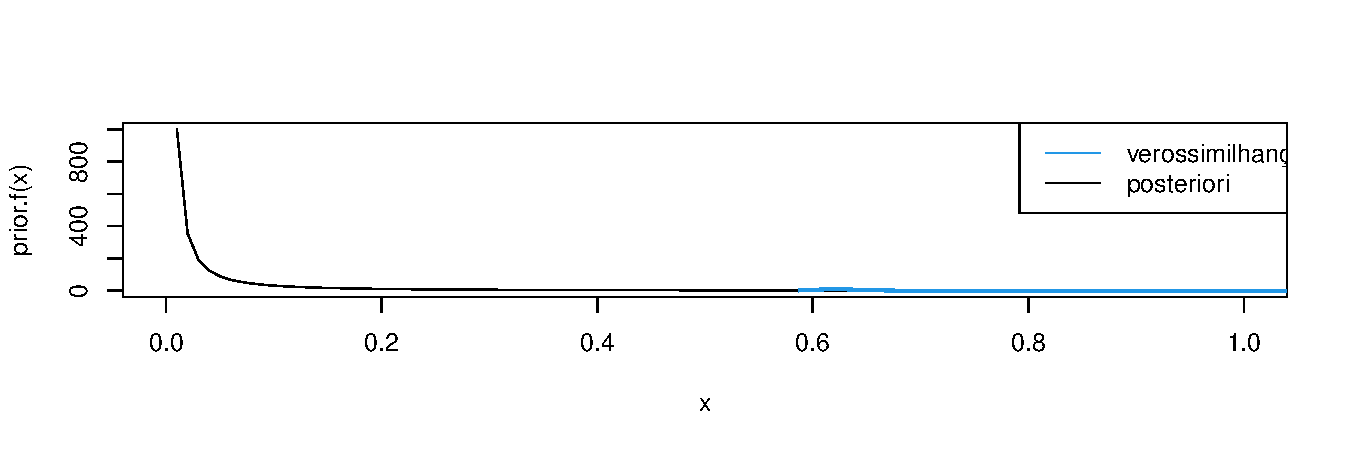
\includegraphics[width=\maxwidth]{figure/pr2-q1-1} 
\begin{kframe}\begin{alltt}
\hlcom{## preditivas (priori e posteriori)}
\hldef{pred0.f} \hlkwb{<-} \hlkwa{function}\hldef{(}\hlkwc{yp}\hldef{)} \hlnum{1}\hlopt{/}\hldef{(yp}\hlopt{+}\hlnum{1}\hlopt{/}\hlnum{2}\hldef{)} \hlcom{## imprória!! ver abaixo}
\hlcom{##pred.f <- function(yp, S, n)}
\hlcom{##    n*exp(lgamma(n+S+1/2) - lgamma(S+1/2) +}
\hlcom{##          lgamma(yp+S+1/2) - lgamma(n+1+yp+S+1/2))}
\hldef{pred.f} \hlkwb{<-} \hlkwa{function}\hldef{(}\hlkwc{yp}\hldef{,} \hlkwc{S}\hldef{,} \hlkwc{n}\hldef{)}
    \hlkwd{exp}\hldef{(}\hlkwd{lbeta}\hldef{(n}\hlopt{+}\hlnum{1}\hldef{, S} \hlopt{+} \hldef{yp} \hlopt{+} \hlnum{0.5}\hldef{)} \hlopt{-} \hlkwd{lbeta}\hldef{(n, S} \hlopt{+} \hlnum{0.5}\hldef{))}
\hldef{yp} \hlkwb{<-} \hlnum{0}\hlopt{:}\hlnum{50}
\hlkwd{plot}\hldef{(yp,} \hlkwd{pred0.f}\hldef{(yp),} \hlkwc{type} \hldef{=} \hlsng{"h"}\hldef{,} \hlkwc{xlab} \hldef{=} \hlsng{"y"}\hldef{,} \hlkwc{ylab} \hldef{=} \hlkwd{TeX}\hldef{(}\hlsng{r"($\textbackslash{}[y_p\textbackslash{}]$)"}\hldef{))}
\end{alltt}


{\ttfamily\noindent\color{warningcolor}{\#\# Warning in charToRaw(str\_replace\_fixed(char, "{}\textbackslash{}\textbackslash{}"{}, "{}"{})): argument should be a character vector of length 1\\\#\# all but the first element will be ignored}}

{\ttfamily\noindent\bfseries\color{errorcolor}{\#\# Error in `str\_replace\_all()`:\\\#\# ! `replacement` function must return a vector the same length as the input (2), not length 1.}}\begin{alltt}
\hlkwd{plot}\hldef{(yp,} \hlkwd{pred.f}\hldef{(yp,} \hlkwc{S} \hldef{= Sy,} \hlkwc{n} \hldef{= ny),} \hlkwc{type} \hldef{=} \hlsng{"h"}\hldef{,} \hlkwc{ylim} \hldef{=} \hlkwd{c}\hldef{(}\hlnum{0}\hldef{,} \hlnum{0.30}\hldef{),}
     \hlkwc{xlab} \hldef{=} \hlkwd{expression}\hldef{(y[p]),} \hlkwc{ylab} \hldef{=} \hlkwd{TeX}\hldef{(}\hlsng{r"($\textbackslash{}[y_p|y\textbackslash{}]$)"}\hldef{))}
\end{alltt}


{\ttfamily\noindent\color{warningcolor}{\#\# Warning in charToRaw(str\_replace\_fixed(char, "{}\textbackslash{}\textbackslash{}"{}, "{}"{})): argument should be a character vector of length 1\\\#\# all but the first element will be ignored}}

{\ttfamily\noindent\bfseries\color{errorcolor}{\#\# Error in `str\_replace\_all()`:\\\#\# ! `replacement` function must return a vector the same length as the input (2), not length 1.}}\begin{alltt}
\hlkwd{sum}\hldef{(}\hlkwd{pred0.f}\hldef{(yp))}                 \hlcom{## imprópria}
\end{alltt}
\begin{verbatim}
## [1] 5.895
\end{verbatim}
\begin{alltt}
\hlkwd{sum}\hldef{(}\hlkwd{pred.f}\hldef{(yp,} \hlkwc{S} \hldef{= Sy,} \hlkwc{n} \hldef{= ny))}  \hlcom{## própria !}
\end{alltt}
\begin{verbatim}
## [1] 0.9979
\end{verbatim}
\begin{alltt}
\hlkwd{require}\hldef{(ggplot2)}
\end{alltt}


{\ttfamily\noindent\itshape\color{messagecolor}{\#\# Carregando pacotes exigidos: ggplot2}}\begin{alltt}
\hlcom{##ggplot() +}
\hlcom{##    xlim(0, 100) +}
\hlcom{##    stat_function(fun = pred.f, args=list(S = Sy, n = ny))}
\hldef{pred} \hlkwb{<-} \hlkwd{data.frame}\hldef{(}\hlkwc{y} \hldef{= yp,} \hlkwc{py} \hldef{=} \hlkwd{pred.f}\hldef{(yp,} \hlkwc{S} \hldef{= Sy,} \hlkwc{n} \hldef{= ny))}
\hlkwd{ggplot}\hldef{(pred)} \hlopt{+}
    \hlkwd{geom_segment}\hldef{(}\hlkwd{aes}\hldef{(}\hlkwc{x}\hldef{=y,}\hlkwc{xend}\hldef{=y,}\hlkwc{y}\hldef{=}\hlnum{0}\hldef{,}\hlkwc{yend}\hldef{=py))} \hlopt{+}
    \hlkwd{theme_bw}\hldef{()}
\end{alltt}
\end{kframe}
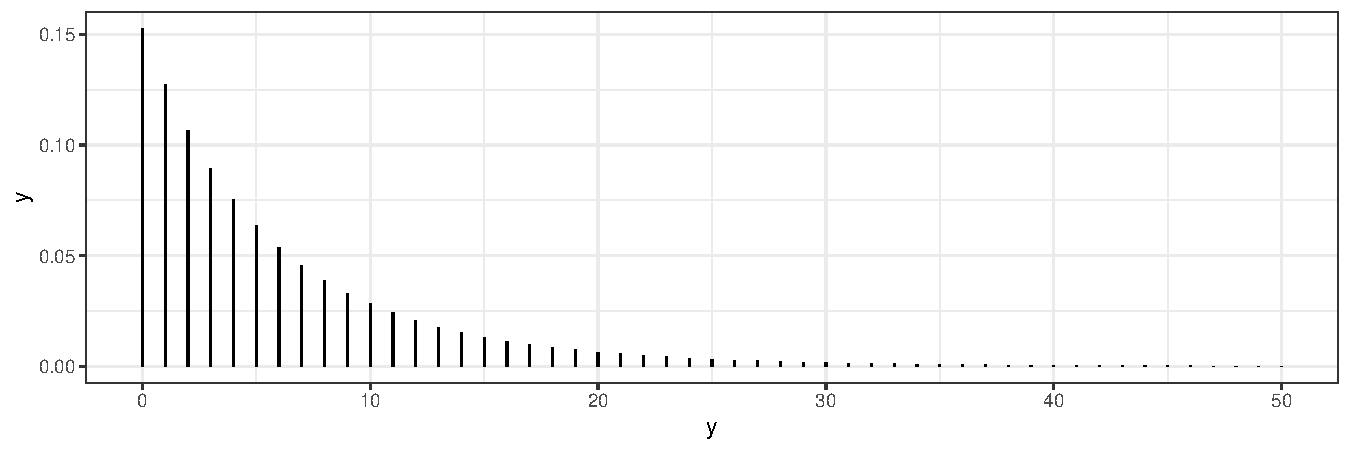
\includegraphics[width=\maxwidth]{figure/pr2-q1-2} 
\end{knitrout}
\end{solucao}

  
\item Embora prioris conjugadas tornem a computação bayesiana
  extremamente simples, elas podem não ser apropriadas e por vezes
  simplesmente não existem (de forma útil) para o modelo que se deseja
  ajustar. Explique como as análises devem ser conduzidas
  neste caso, descrevendo pelo menos duas abordagens.

\begin{extra}
{\it Implemente as abordagens mencionadas. (sugestão: implementar ao menos a aproximação gaussiana e MCMC).}
\end{extra}

\begin{solucao}

\end{solucao}


\item Vai se modelar o número diário de acidentes em um trecho de rodovia com o modelo Poisson
  com priori "half-normal". Mostre a expressão da posteriori (a uma constante) e indique se é (ou não) compatível com alguma distribuição conhecida.
  Opta-se por fazer uma análise com aproximação discreta de cinco pontos.
  O conjunto de dados é $0, 3, 2, 1, 0, 2$.
  Escolha cinco pontos razoáveis e obtenha a posteriori (discreta) e calcule a sua média e moda.

\begin{extra}
  {\it Após obter a solução escrita implemente em um código. Faça inicialmente a aproximação de 5 pontos e depois obtenha a discretização com mais pontos.
  Escreva também uma função para posteriori que inclua o cálculo da constante normalizadora por integração numérica. }
\end{extra}
  
\begin{solucao}


\end{solucao}

  
\item Considere um modelo Gama para a distribuição de uma amostra aleatória de uma variável, ou seja,
  \[ f(y|\alpha, \beta) = \frac{\beta^\alpha}{\Gamma(\alpha)} y^{\alpha-1} \exp\{-\beta y\} . \]
Considere ainda prioris também Gama, independentes, para cada parâmetro.
\begin{enumerate}
  \item Obtenha a expressão da posteriori conjunta, a uma constante de proporcionalidade.
  \item Indique como pode ser obtida a distribuição posteriori marginal de cada parâmetro, isto é, $f(\alpha|y)$ e $f(\beta|y)$. 
  \item Obtenha a distribuição posteriori condicional de cada parâmetro, isto é, $f(\alpha|\beta, y)$ e $f(\beta|\alpha, y)$. 
  \item Explique como seriam poderiam ser obtidas amostras da posteriori neste caso. %, (i) por simulação direta da posteriori (ii) pelo algorítmo de Gibbs.
%  \item Neste exemplo, nos passos do Gibbs as amostras são obtidas diretamente de alguma distribuição conhecida ou é necessário usar algum algorítmo de rejeição (MCMC ou algum outro)? Justifique. 
\end{enumerate}

\begin{extra}
  {\it Escolha valores dos hiperparâmetros do modelo e produza gráficos das prioris $f(\alpha)$, $f(\beta)$ e da conjunta
    $f(\alpha, \beta)$. Use o modelo especificado para gerar uma amostra de $n = 12$ valores. Obtenha gráficos dos itens a) a c).
    Obtenha amostras da posteriori conforme item d). Faça o histograma das amostras obtidas e sobreponha com a densidade (marginal) teórica.}
\end{extra}

\begin{solucao}

\end{solucao}



\item Foi visto que distribuições da família exponencial, isto é,  podem ser escritas na forma
  \[ f(y|\theta) = h(y) g(\theta) \exp\{t(y) c(\theta)\}, \] 
  possuem prioris conjugadas.
  Use este resultado para obter, a partir da notação de família exponencial,
  a priori conjugada para uma amostragem de $Y \sim {\rm Gama}(a, \theta)$
  em que $a$ é conhecido e $\theta$ é o 
  parâmetro desconhecido sobre o qual deseja-se fazer inferência.
  Quais as quantidades amostrais (suficientes) necessárias para inferência?

% \begin{extra}
% {\it }
% \end{extra}
    
\item Seja $Y|\theta \sim {\rm Bin}(n, \theta)$ a priori de $\theta$ uma mistura das distribuições ${\rm Beta}(1, 3)$ e $ {\rm Beta}(5, 2)$ com pesos 2/3 e 1/3, respectivamente. Uma amostra forneceu $y = 3, n = 9$. Esboce os gráficos de cada um de seus componentes da priori. Obtenha a expressão da posteriori e um esboço do seu gráfico.

\begin{extra}
{\it Obtenha os gráficos para priori e suas componentes, da verossimilhança e da posteriori. }
\end{extra}

\begin{solucao}
\begin{knitrout}
\definecolor{shadecolor}{rgb}{0.969, 0.969, 0.969}\color{fgcolor}\begin{kframe}
\begin{alltt}
\hldef{dpriori} \hlkwb{<-} \hlkwa{function}\hldef{(}\hlkwc{theta}\hldef{) (}\hlnum{1}\hlopt{/}\hlnum{3}\hldef{)}\hlopt{*}\hlkwd{dbeta}\hldef{(theta,} \hlnum{1}\hldef{,} \hlnum{3}\hldef{)} \hlopt{+} \hldef{(}\hlnum{2}\hlopt{/}\hlnum{3}\hldef{)}\hlopt{*}\hlkwd{dbeta}\hldef{(theta,} \hlnum{5}\hldef{,} \hlnum{2}\hldef{)}
\hldef{ap} \hlkwb{<-}  \hlkwa{function}\hldef{(}\hlkwc{x}\hldef{,} \hlkwc{w}\hldef{,} \hlkwc{a}\hldef{,} \hlkwc{b}\hldef{,}\hlkwc{...}\hldef{) w}\hlopt{*}\hlkwd{dbeta}\hldef{(x, a, b)}
\hlkwd{curve}\hldef{(}\hlkwd{ap}\hldef{(x,} \hlnum{1}\hlopt{/}\hlnum{3}\hldef{,} \hlnum{1}\hldef{,} \hlnum{3}\hldef{),} \hlkwc{lty} \hldef{=} \hlnum{2}\hldef{,} \hlkwc{col} \hldef{=} \hlnum{2}\hldef{,} \hlkwc{ylim} \hldef{=} \hlkwd{c}\hldef{(}\hlnum{0}\hldef{,} \hlnum{3.5}\hldef{))}
\hlkwd{curve}\hldef{(}\hlkwd{ap}\hldef{(x,} \hlnum{2}\hlopt{/}\hlnum{3}\hldef{,} \hlnum{5}\hldef{,} \hlnum{2}\hldef{),} \hlkwc{lty} \hldef{=} \hlnum{2}\hldef{,} \hlkwc{col} \hldef{=} \hlnum{2}\hldef{,} \hlkwc{add} \hldef{=} \hlnum{TRUE}\hldef{)}
\hlkwd{curve}\hldef{(}\hlkwd{dpriori}\hldef{(x),} \hlkwc{col} \hldef{=} \hlnum{2}\hldef{,} \hlkwc{add} \hldef{=} \hlnum{TRUE}\hldef{)}
\hlcom{##}
\hldef{n} \hlkwb{<-} \hlnum{9}\hldef{; y} \hlkwb{<-} \hlnum{3}
\hlkwd{curve}\hldef{(}\hlkwd{dbeta}\hldef{(x,} \hlnum{10}\hldef{,} \hlnum{7}\hldef{),} \hlkwc{col} \hldef{=} \hlnum{4}\hldef{,} \hlkwc{add} \hldef{=} \hlnum{TRUE}\hldef{)}
\hlcom{##}
\hldef{w1} \hlkwb{<-} \hldef{(}\hlnum{1}\hlopt{/}\hlnum{3}\hldef{)}\hlopt{*}\hlkwd{beta}\hldef{(}\hlnum{1}\hlopt{+}\hlnum{3}\hldef{,} \hlnum{3}\hlopt{+}\hldef{(}\hlnum{9}\hlopt{-}\hlnum{3}\hldef{))}\hlopt{/}\hlkwd{beta}\hldef{(}\hlnum{1}\hldef{,}\hlnum{3}\hldef{)}
\hldef{w2} \hlkwb{<-} \hldef{(}\hlnum{2}\hlopt{/}\hlnum{3}\hldef{)}\hlopt{*}\hlkwd{beta}\hldef{(}\hlnum{5}\hlopt{+}\hlnum{3}\hldef{,} \hlnum{2}\hlopt{+}\hldef{(}\hlnum{9}\hlopt{-}\hlnum{3}\hldef{))}\hlopt{/}\hlkwd{beta}\hldef{(}\hlnum{5}\hldef{,}\hlnum{2}\hldef{)}
\hldef{p1s} \hlkwb{<-} \hldef{w1}\hlopt{/}\hldef{(w1}\hlopt{+}\hldef{w2)}
\hldef{p2s} \hlkwb{<-} \hldef{w2}\hlopt{/}\hldef{(w1}\hlopt{+}\hldef{w2)}
\hldef{dpost} \hlkwb{<-} \hlkwa{function}\hldef{(}\hlkwc{theta}\hldef{) (p1s)}\hlopt{*}\hlkwd{dbeta}\hldef{(theta,} \hlnum{1}\hlopt{+}\hlnum{3}\hldef{,} \hlnum{3}\hlopt{+}\hldef{(}\hlnum{9}\hlopt{-}\hlnum{6}\hldef{))} \hlopt{+}
                             \hldef{(p2s)}\hlopt{*}\hlkwd{dbeta}\hldef{(theta,} \hlnum{5}\hlopt{+}\hlnum{3}\hldef{,} \hlnum{2}\hlopt{+}\hldef{(}\hlnum{9}\hlopt{-}\hlnum{6}\hldef{))}
\hlkwd{curve}\hldef{(}\hlkwd{dpost}\hldef{(x),} \hlkwc{add} \hldef{=} \hlnum{TRUE}\hldef{)}
\end{alltt}
\end{kframe}
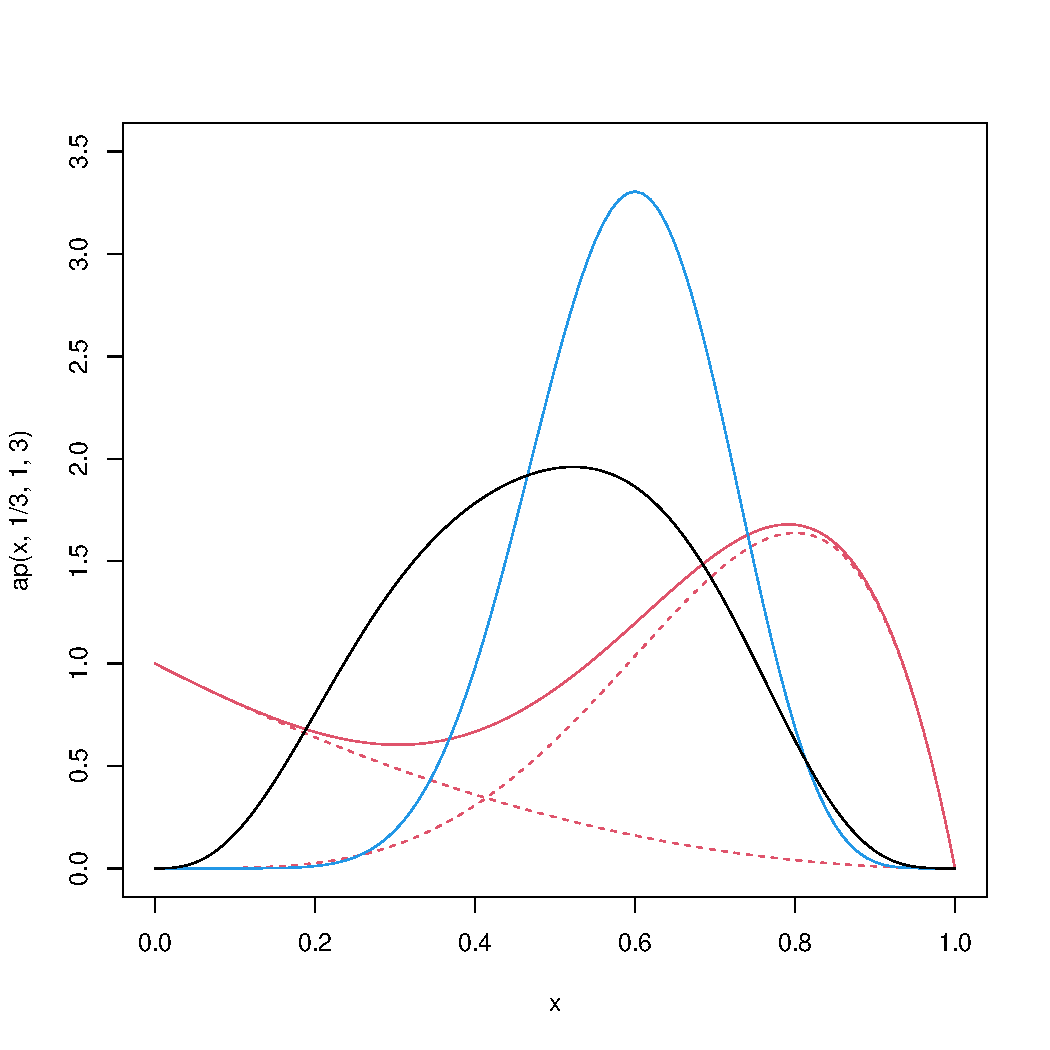
\includegraphics[width=\maxwidth]{figure/unnamed-chunk-14-1} 
\end{knitrout}
\end{solucao}


%\newpage
  
\item A classificação de qualidade de um componente elétrico é excelente ($y = 1$), bom ($y = 2$) ou ruim ($y = 3$). A probabilidade de vários níveis de qualidade dependem da fábrica onde é produzido ($\theta_1 = 0$: fábrica A, $\theta_1 = 1$: fábrica B) e do tipo de máquina ($\theta_2 = 0$: máquina I, $\theta_2 = 1$: máquina II, $\theta_2 = 2$: máquina III). As probabilidades para $y = 2$ são dadas pela Tabela~\ref{tab:exerc1a-cap4}.
Além disso, distribuição conjunta de $(\theta_1, \theta_2)$ é dada na Tabela~\ref{tab:exerc1b-cap4}.
Encontre a distribuição posteriori conjunta de $\theta_1, \theta_2|y = 2$ e cada uma das distribuições marginais. Tendo observado $y = 2$:
(a) qual a combinação fábrica/máquina é a mais provável de ter produzido esse componente? (b) Qual a posteriori (conjunta)? (c) Quais são as marginais? (d) E as condicionais?  


\begin{table}[ht!]
\centering
\caption{Probabilidades condicionais $y = 2$}
\label{tab:exerc1a-cap4}
  \begin{tabular}{c| c c}
    Pr($y = 2|\theta_1, \theta_2$)         &$\theta_1 = 0$          &$\theta_1 =1$\\
    \hline
    $\theta_2 = 0$                         &0,3                    &0,2\\
    $\theta_2 = 1$                         &0,4                    &0,2\\
    $\theta_2 = 2$                         &0,6                    &0,3\\
    \hline
  \end{tabular}
\end{table}

\begin{table}[ht!]
\centering
\caption{Probabilidade a priori das combinações fábrica/máquina}
\label{tab:exerc1b-cap4}
  \begin{tabular}{c| c c}
    Pr($\theta_1, \theta_2$)               &$\theta_1 = 0$          &$\theta_1 =1$\\
    \hline
    $\theta_2 = 0$                         &0,1                    &0,2\\
    $\theta_2 = 1$                         &0,2                    &0,3\\
    $\theta_2 = 2$                         &0,1                    &0,1\\
    \hline  
\end{tabular}
\end{table}

%\begin{extra}
%{\it Obtenha gráficos da priori, verossimilhança e posteriori deste problema.}
%\end{extra}

\begin{solucao}
\end{solucao}


\item Um conjunto $y_1, y_2, \ldots, y_n$ é {\tt permutável} ({\it exchangeable}) se a probabilidade conjunta  $f(y_1, y_2, \ldots, y_n)$ é invariante a uma permutação $\pi$ dos índices,
  ou seja,  $f(y_1, y_2, \ldots,y_n) = f(\pi(y_1), \pi(y_2), \ldots, \pi(y_n))$ para qualquer permutação $\pi$ dos índices.

  Um conjunto $y_1, y_2, \ldots, y_n$ é {\tt independente} se a probabilidade conjunta  $f(y_1, y_2, \ldots, y_n)$ é fatorável  $f(y_1, y_2, \ldots, y_n) =  f(y_1) \cdot f(y_2) \cdot f(y_n)$. Desta forma, para $n=2$ isto implica que $f(y_2|y_1) = f(y_2)$

Considere uma urna com uma bola branca e uma preta com probabilidade 1/2 de retirar cada uma delas. As bolas serão retiradas da urna sem reposição. Mostre que as variáveis definidas pelos resultados das retiradas são permutáveis, mas não independentes.

Dica de notação: Denote a primeira bola ser branca por $Y_1 = 0$  e preta por $Y_1 = 1$. Use análogo para segunda bola.  

\begin{solucao}
São permutáveis pois 
\[ 1/2 = P(Y_1 = 1, Y_2 = 0) = P(Y_1 = 0, Y_2 = 1) = 1/2, \]
mas não são independentes pois
\[0 = P(Y_2 = 1|Y_1 = 1) \neq P[Y_2 = 1] = 1/2 \]
\end{solucao}
    
%%%
%%% $1^a$ Prova (17/10/2024)
%%%
  
\item  \textit{
Em um grupo de estudantes 55\% são do curso $A$, 35\% do curso $B$ o restante do
curso $C$. A proporção estudantes que estão fazendo a segunda graduação em cada um dos cursos é de 5, 10  e 25\%, respectivamente. 
Se um estudante é sorteado ao acaso e verifica-se que está fazendo a segunda graduação, qual a probabilidade de
ser de cada um dos cursos?}
\begin{enumerate}
\item A qual curso voce arriscaria dizer que o estudante sorteado pertence? Justifique.
\item Resolva a problema da forma que achar adequada.
\item Considere agora o problema do ponto de vista Bayesiano.
  Qual é a variável resposta $(Y)$ e sua distribuição?
  Qual é o parâmetro $(\theta)$ e sua distribuição a {\it priori}?
 Qual a verossimilhança? E a {\it posteriori}? E a marginal (preditiva)?
\item Esboce um gráfico da {\it priori} e da {\it posteriori}.
\item Interprete os resultados.
\item Agora que resolveu o problema, em qual curso ``apostaria'' que  o estudante pertence? Justifique
\end{enumerate}

\item Suponha que o tempo em minutos necessário para atender um cliente em um banco possui uma distribuição exponencial com parâmetro $\theta$.
  Para fins de planejamento de serviços deseja-se conhecer melhor o processo, o que é feito por  inferências sobre $\theta$.
  Baseada em conhecimento prático e subjetivo, a incerteza sobre $\theta$ é descrita por uma distribuição (\textit{a priori}) de probabilidades para os tempos de atendimento.
  Para conhecer melhor o processo vai se coletar uma amostra registrando o tempo gasto em $n$ atendimentos.
  \begin{enumerate}
  \item Escreva a função de probabilidades para as observações.
  \item Escreva a função de verossimilhança. 
  \item Reconheça uma distribuição de probabilidades proporcional à esta expressão da verossimilhança. Qual é a distribuição e com quais valores de parâmetros? 
  \item Forneça a expressão de uma distribuição à {\it priori} conjugada.
  \item Qual(ais) valor(es) você especificaria para o(s) parâmetro(s) da distribuição {\it priori} conjugada (hiperparâmetros)? Justifique.
  \item Obtenha a expressão da distribuição marginal (preditiva a priori).
  \item Explique como faria para simular valores desta distribuição marginal.
  \item Obtenha a expressão da posteriori e indique qual a distribuição de probabilidades.
  \item Qual(ais) quantidade(s) calculada(s) com a amostra são necessárias para a obtenção da verossimilhança e posteriori?
  \item O estudo foi feito em uma primeira agência e o tempo médio observado para atender 20 clientes foi de 10,5 minutos. Forneça a expressão da distribuição a posteriori para $\theta$ com estes valores.
  \item Qual o valor esperado da distribuição a posteriori para $\theta$?
  \item Mostre que o valor esperado da posterior é uma média ponderada entre o valor esperado da priori e do estimador de máxima verossimilhança (inverso da média dos dados). 
  \item Qual seria a distribuição preditiva para uma nova observação após obter esta primeira amostra?
  \item Qual o valor esperado da distribuição marginal $[Y]$?
  \item Em uma segunda agência, o estudo foi feito com 12 clientes e o tempo médio de atendimento foi de 8,5 minutos. Qual a posteriori após considerar os dados desta segunda agência?
  \item Após algum tempo decidiu-se por igualar os tamanhos das amostras e completou-se a amostra da segunda agência anotando-se os tempos de atendimento de mais oito clientes que totalizaram 108 minutos. Compare os resultados da primeira agência e da segunda após esta complementação da amostra.
  \end{enumerate}

  \newpage

% \item Indique para cada trecho de código a seguir o modelo usado e o que está sendo obtido.
  
%   \begin{enumerate}
% \item
% <<eval = FALSE>>=
% vec1 <- rgamma(1E5, shape = 10, rate = 3)
% vec2 <- rexp(1E5, rate = vec1)
% hist(vec2, freq = FALSE, nclass = 30)
% @ 
% % \item
% % <<eval = FALSE>>=
% % ## ... continuando anterior
% % mean(vec1)
% % 10/3
% % @
% \item
% <<eval = FALSE>>=
% vec1 <- rgamma(1E6, shape = 5, rate = 2)
% vec2 <- rpois(1E6, lambda = vec1)
% hist(vec1[vec2 == 5], freq = FALSE, nclass = 30)
% @
% \item
% <<eval = FALSE>>=
% curve(dbeta(x, 2, 8), ylim = c(0, 7))
% curve(dbeta(x, 2 + 10, 8 + 30), col = 4, add = TRUE)
% @ 
% \item
% <<eval = FALSE>>=
% ## ... continuando anterior
% vec1 <- rbeta(1E5, 2 + 10, 8 + 30)
% vec2 <- rbinom(1E5, size = 1, prob = vec1)
% prop.table(table(vec2))
% @
% \end{enumerate}

\item Forneça a expressão da priori conjugada dos seguintes modelos de $[Y|\theta]$. Justifique as respostas.
  \begin{enumerate}
  \item ${\rm Geometrica}(\theta)$
  \item ${\rm Gama}(a = 5, \theta)$
  \item ${\rm Normal}(\mu = 100, \theta)$
  \item ${\rm Weibull}(\alpha = 2, \theta)$
  \item ${\rm Normal}(\theta, \sigma = 1)$    
\end{enumerate}

% \item Escreva de maneira suscinta (um parágrafo com no máximo 10 linhas) como voce explicaria para um pesquisador de outra área as características da análise bayesiana em contraste com outra(s) abordagem(ens) para inferência estatística.


  %%% 
  %%% 2022 2a prova (05/05/2022)
  %%% 
  
\item Comente sobre intervalos HPD frequentemente usados em inferência
  bayesiana em contraste com intervalos assintóticos e baseados em
  quantis, apontando as principais características e diferenças.

\item Embora prioris conjugadas tornem a computação bayesiana
  extremamente simples, elas podem não ser apropriadas e por vezes
  simplesmente não existem (de forma útil) para o modelo que se deseje
  ajustar. Explique com detalhes como as análises devem ser conduzidas
  neste caso, considerando pelo menos duas abordagens (de natureza
  distinta).


\item Suponha que em um experimento físico, a variação temporal de uma
  corrente elétrica, denotada por $X$, tem distribuição uniforme no
  intervalo $[0,\theta]$. Sendo $X_1,\cdots,X_n$ realizações aleatórias
  desse experimento e assumindo o seguinte modelo a priori para $\theta$
\[
\pi(\theta) = \frac{10}{\theta^{11}}\underset{{[1,\infty)}}{ \mathbb{I}(\theta)},
\]
pede-se
\begin{enumerate}
	\item[a)] Mostre que a distribuição a posteriori de $\theta$ é dada por
\[
\pi(\theta|X_1,\cdots,X_n) = \frac{(n + 10 )\theta_0^{n + 10 }}{\theta^{n+11}}\underset{{[\theta_0,\infty)}}{ \mathbb{I}(\theta)},
\]
sendo $\theta_0 = {\rm max}\left\{X_{(n)},1\right\} $ para $X_{(n)} = {\rm max}\left\{X_1,\cdots,X_n\right\}$.
	\item[b)] Obtenha o estimador de Bayes sob perda $0-1$ de $\theta$.\\
	{\it {\bf Dica}: Qual o valor de $\theta$ que fornece o maior valor de $\pi(\theta|X_1,\cdots,X_n)$?}

	\item[c)] Obtenha o intervalo HPD com $90\%$ de credibilidade de $\theta$.\\
	{\it {\bf Dica}: Note que $\pi(\theta|X_1,\cdots,X_n)$ é unimodal e decrescente em $\theta$.}
\end{enumerate}


\begin{solucao}

 {\it Solução}:

-- {\bf item a)} Temos
\[
\begin{split}
\pi(\theta|X_1,\cdots,X_n) & \propto \left[ \prod_{i=1}^{n} \frac{1}{\theta} \underset{{[0,\theta)}}{ \mathbb{I}(x_i)}\right] \frac{1}{\theta^{11}}\underset{{[1,\infty)}}{ \mathbb{I}(\theta)}\\
& = \frac{1}{\theta^{n + 11}}  \prod_{i=1}^{n} \underset{{[0,\theta)}}{ \mathbb{I}(x_i)} \underset{{[1,\infty)}}{ \mathbb{I}(\theta)}.
\end{split}
\]
Note que todos os $X_i$'s são menores que $\theta$. Em particular, o valor máximo dos $X_i$'s é menor do que $\theta$. Isso sugere que, condicional a $X_{(n)}$, os demais $X_i$'s não trazem informação sobre $\theta$. Portanto
\[
\pi(\theta|X_1,\cdots,X_n)  \propto \frac{1}{\theta^{n + 11}}   \underset{{[x_{(n)},\infty)}}{ \mathbb{I}(\theta)}   \underset{{[1,\infty)}}{ \mathbb{I}(\theta)}.
\]
De modo que
\[
\underset{{[x_{(n)},\infty)}}{ \mathbb{I}(\theta)}   \underset{{[1,\infty)}}{ \mathbb{I}(\theta)} \left\{\begin{array}{l}
	1,\;\mbox{se $\theta \geq \theta_0$}\\
	0,\;\mbox{caso contrário.}
\end{array} \right.
\]
Portanto
\[
\pi(\theta|X_1,\cdots,X_n)  \propto \frac{1}{\theta^{n + 11}} \underset{{[\theta_0,\infty)}}{ \mathbb{I}(\theta)}.
\]
Agora precisamos calcular a constante $c$ tal que
$$\int_{-\infty}^{\infty} c\; \frac{1}{\theta^{n + 11}} \underset{{[\theta_0,\infty)}}{ \mathbb{I}(\theta)} d\theta = 1$$.
Resolvendo essa desigualdade, temos $c = (10 + n)\theta_0^{10 + n}$. Conclui-se assim, que
\[
\pi(\theta|X_1,\cdots,X_n) = \frac{(n + 10 )\theta_0^{n + 10 }}{\theta^{n + 11}}\underset{{[\theta_0,\infty)}}{ \mathbb{I}(\theta)}.
\]

-- {\bf item b)} A função densidade $\pi(\theta|X_1,\cdots,X_n)$ é contínua e decrescente em $\theta$, portanto o estimador de Bayes sob perda $0-1$ é $\theta_0$.


-- {\bf item c)} Como a função densidade $\pi(\theta|X_1,\cdots,X_n)$ é contínua e decrescente em $\theta$, o intervalo HPD para $\theta$ é da forma $[\theta_0,a]$, onde $a$ é o quantil que deixa uma área de $10\%$ a direita. Assim, precisamos encontrar o valor $a$ que satisfaz:
\[
\int_{a}^{\infty} \frac{(n + 10 )\theta_0^{n + 10 }}{\theta^{n + 11}} d\theta = 0,1.
\]
Segue que
\[
\begin{split}
	\int_{a}^{\infty} \frac{(n + 10 )\theta_0^{n + 10 }}{\theta^{n + 11}} d\theta &= \left.(n + 10 )\theta_0^{n + 10 } \frac{\theta^{-(n + 11)+ 1}}{-(n + 11)+ 1}\right|_{\theta=a}^{\theta=\infty}= (n + 10 )\theta_0^{n + 10 } \frac{a^{-(n + 10)}}{n + 10} = 0,1\;\; (\Leftrightarrow)\\
	a^{(n + 10)} &= 10\theta_0^{(n + 10)} \;\;\hspace{10cm} (\Leftrightarrow)\\
	a &= 10^{1/(n + 10)} \theta_0.
\end{split}
\]
Portanto, o intervalo HPD com $90\%$ de credibilidade de $\theta$ é dado por $[\theta_0\,,\,10^{1/(n + 10)} \theta_0]$

\end{solucao}

\item Seja $X_1, \ldots, X_n$ uma amostra aleatória de uma distribuição com função de probabilidades:
\[ f(x|\theta) = \theta \exp\{-\theta x\},\;\mbox{ com  } x > 0\mbox{  e  } \theta > 0.  \]
Suponha o modelo a priori de Jeffreys para $\theta$ (ou seja, $\pi (\theta) \propto 1/\theta,\,\theta > 0$). Com isso, considere o teste de hipóteses: ${\rm H_0}: \theta \leq 1$ vs ${\rm H_1}: \theta > 1$.
\begin{enumerate}
\item Obtenha o modelo a posteriori de $\theta$, e expresse o
  estimador de Bayes sob perda quadrática para $\theta$.
\item Supondo $\sum_{i=1}^{n} x_i = 1,5$, decida sobre ${\rm H_0}$ contra ${\rm H_1}$ considerando a seguinte estrutura de perda
  \begin{table}[!htb]
    \centering
    \begin{tabular}{c|cc}
      \hline
      \multirow{2}{*}{$L(\theta, a)$}& \multicolumn{2}{c}{Decisão} \\
                                     & $\theta \leq 1$ & $\theta > 1$ \\
      \hline
      $\theta \leq 1$& 0 & $1$ \\
      $\theta > 1$& $ 1 $& 0 \\
      \hline
    \end{tabular}
  \end{table}

  Considere $n=10$ e expresse os comandos em R para obter a resposta.

  % \item Repita o item anterior usando fator de Bayes, e expresse os comandos em R para obter a resposta.

\end{enumerate}

\item Em algoritmos de MCMC, para se verificar se as cadeias
  atingiram a distribuição estacionária (convergência), é útil
  verificar se as diferentes cadeias já se misturaram a ponto de se
  tornarem indistinguíveis. Para isso é necessário dispor de
  múltiplas cadeias e utilizar pontos de partida bastante dispersos.
  O teste de Gelman-Rubin calcula a estatística $\hat{R}$
  (\texttt{Rhat}), definida como
  $$
  \hat{R} = \frac{S}{W}
  $$
  sendo $S$ o desvio padrão calculado a partir da mistura de todas as
  cadeias, e $W$ a média dos desvios padrão das cadeias indivíduais.
  Valores de $\hat{R}$ muito maiores do que 1 são indicação de que ainda
  não houve convergência. A medida que as cadeias evoluem, o valor de
  $\hat{R}$, tende a se aproximar de 1. Como regra geral, considera-se
  aceitável valores $\hat{R} < 1.05$. Outra questão pertinente é saber
  se a informação contida na amostra simulada é suficiente. Ou seja,
  desejamos saber se o tamanho $n_s$ da amostra simulada da distribuição
  posterior de fato tem a acurácia de uma amostra de $n$ elementos
  independentes. Essa questão se justifica pelo fato de que os valores
  gerados nas cadeias tendem a apresentar autocorrelação. Uma forma de
  verificar esse fato se dá por meio do cálculo do número efetivo de
  amostras (\texttt{n.eff})
  $$
  n_{eff} = \frac{1}{1 + 2 \sum_{i=1}^{\infty} \rho_k}
  $$
  onde $\rho_k$ são as correlações para o espaçamento de $k$ passos na
  cadeia. Quanto mais próximo $n_{eff}$ estiver de $n$, melhor.

  O resultado abaixo é o resumo da distribuição posterior para o
  parâmetro $\theta$ de uma distribuição Binomial com $n = 3000$, obtido
  via JAGS
\begin{verbatim}
          mean    sd  2.5%   50% 97.5% [...]  Rhat n.eff
theta    0.163 0.136 0.006 0.129 0.508 [...] 1.12    752
\end{verbatim}
  Com esse resultado, comente sobre os valores obtidos de \texttt{Rhat}
  e \texttt{n.eff}, e o que deveria ser feito para que esses valores
  fiquem mais adequados.




\item Descreva o modelo sendo ajustado, distribuições envolvidas, parâmetros e constantes.
  Esboce ainda a estrutura dos dados nas seguintes declarações de modelos em JAGS.

  \begin{enumerate}
  \item
\begin{verbatim}
model{
  for (i in 1:N){
    x[i] ~ dbern(p)
  }
  p ~ dbeta(alpha, beta)
  alpha <- 1
  beta <- 1
}
\end{verbatim}

  \item
\begin{verbatim}
model{
  for(i in 1:M){
     for(j in 1:N){
        y[i,j] ~ dnorm(mu[i], tau)
     }
     mu[i] ~ dnorm(theta, tauD)
  }
  tau <- pow(sigma, -2)
  sigma ~ dunif(0, 100)
  theta ~ dnorm(0, .001)
  tauD <- pow(delta, -2)
  delta ~ dunif(0, 100)
}
\end{verbatim}


  \item
\begin{verbatim}
model{
  for (i in 1:N){
    y[i] ~ dbern(p[i])
    logit(p[i]) <- a[g[i]] * x[i]
  }
  for (j in 1:K){
    a[j] ~ dnorm(mu.a, tau.a)
  }
  mu.a ~ dnorm(0, 0.0001)
  tau.a <- pow(sigma.a, -2)
  sigma.a ~ dunif(0, 1000)
}
\end{verbatim}

  \item
\begin{verbatim}
model{
  for (i in 1:N){
    y[i] ~ dnorm(mu[i], tau)
    mu[i] <- a[g[i]] * x[i] + b[g[i]]
  }
  for (j in 1:K){
    a[j] ~ dnorm(mu.a, tau.a)
    b[j] ~ dnorm(mu.b, tau.b)
  }
  mu.a ~ dnorm(0, 0.0001)
  mu.b ~ dnorm(0, 0.0001)
  tau <- pow(sigma, -2)
  sigma ~ dunif(0, 1000)
  tau.a <- pow(sigma.a, -2)
  tau.b <- pow(sigma.b, -2)
  sigma.a ~ dunif(0, 1000)
  sigma.b ~ dunif(0, 1000)
}
\end{verbatim}

  \item
\begin{verbatim}
model{
  for (t in 1:T) {
    y[t] ~ dbeta(a[t], b[t])
    a[t] <- mu[t] * phi
    b[t] <- (1 - mu[t]) * phi
    logit(mu[t]) <- alpha + beta * x[t]
  }
  alpha ~ dnorm(0, 10^-2)
  beta ~ dnorm(0, 10^-2)
  phi ~ dunif(0, 10)
}

\end{verbatim}

  \item
\begin{verbatim}
model
{
  for (i in 1:T) {
    y[i] ~ dbin(p[i], K)
    logit(p[i]) <- alpha + beta_1 * x_1[i] + beta_2 * x_2[i]
  }
  alpha ~ dnorm(0.0,0.01)
  beta_1 ~ dnorm(0.0,0.01)
  beta_2 ~ dnorm(0.0,0.01)
}
\end{verbatim}

  \item
\begin{verbatim}
model{
  for(i in 1:n){
      y[i] ~ dpois(mu[i])
      mu[i] <- ifelse(i > k, lambda, theta)
  }
  k ~ dcat(ano[]) # distribuição para dados categóricos ou discretos
  theta ~ dgamma(a1, b1)
  lambda ~ dgamma(a2, b2)
  dif <- lambda - theta
  ib1 ~ dgamma(c1, d1)
  b1 <- 1/ib1
  ib2 ~ dgamma(c2, d2)
  b2 <- 1/ib2
  a1 <- 0.5
  a2 <- 0.5
  c1 <- 0.1
  c2 <- 0.1
  d1 <- 1
  d2 <- 1
}
\end{verbatim}

  \end{enumerate}

  %%%
  %%% 2022 1a prova (17/03/2022)
  %%%

\item{ Com base no que você viu no curso até agora, responda:
    \begin{enumerate}
    \item Usando apenas palavras, como você explicaria para um leigo o
      que é inferência bayesiana?
    \item Usando notação estatística, como você explicaria para um
      estatístico (mas que não sabe ainda) o que é inferência bayesiana?
    \item Quais são as principais diferenças entre a inferência clássica
      (frequentista e por verossimilhança) e a inferência bayesiana?
      (Por exemplo, para cada uma: qual é o objeto de inferência? Quais
      as suposições feitas sob os parâmetros? Como os dados são
      tratados? Como as informações prévias podem ser consideradas?)
    \item O que você julga serem os pontos fortes e fracos da inferência
      bayesiana?
    \end{enumerate}
  }


% \item Seja $y_1, \ldots, y_n$ uma amostra aleatória de uma distribuição com função probabilidades:
% \[ f(y|\theta) = \theta \exp\{-\theta y\} \]
% Obtenha a priori de Jeffreys,
% a expressão da posteriori, da marginal e da distribuição preditiva.


% \item No contexto do problema anterior imagine que está se medindo o tempo para atender clientes em um banco.
%   Forneça as expressões caso seja assumida como priori uma distribuição gama de média 0,25 e desvio padrão 1.
%   Além disto considere que foi observada uma amostra aleatória de 20 tempos de atendimento e o tempo médio dos dados
%   desta amostra foi de 4,8 minutos.

% \item Forneça os comandos para desenhar em um gráfico as curvas da priori, verossimilhança e posteriori do item anterior.

%%
%% 2019 Prova 1
%%
\item Decidiu-se examinar um conjunto de imagens médicas tomadas independentemente
  de diferentes indivíduos. O objetivo é fazer inferências sobre a proporção de imagens 
  com determinada característica morfológica.
  Em particular deseja-se avaliar se a proporção de indivíduos com alteração está
  abaixo de 40\%.
\begin{itemize}
  \item Em um primeiro estudo tomaram-se 9 imagens sendo detectadas 3 com alteração.
  \item Em um segundo estudo decidiu-se tomar-se imagens até que se obtivesse 3 com
    alteração. Ocorreu que foram tomadas 9 imagens no total.
\end{itemize}
\begin{enumerate}
\item  Como seria testada a hipótese de interesse em cada estudo no enfoque não Bayesiano?
\item Neste caso os dois estudos forneceriam a mesma conclusão estatística?
\item Em uma análise Bayesiana com uma priori $[\theta] \sim {\rm Be}(1,5 ; 1,5)$,
  qual seria a posteriori em cada estudo? 
\item Como deveria ser avaliada a posteriori para concluir sobre a hipótese de interesese?
  Os estudos produziriam a mesma conclusão estatística? Justifique.
\item Se alternativamente decide-se adotar a priori de Jeffreys em cada estudo, 
  elas seriam as mesmas a produziram a mesma posteriori? Justifique. 
\end{enumerate}


\item Uma empresa adquire 30\% de sua matéria prima de um primeiro fornecedor, 50\% de um segundo e o restante de um terceiro fornecedor.
Os lotes de matéria prima são inspecionados e, se considerados não satisfatórios, são enviados de volta.
Sabe-se que 2\%, 5\% e 1\% dos lotes são retornados a cada fornecedor, respectivamente.
Rejeitando-se um lote, deseja-se quantificar a chance de ter vindo de cada um dos fornecedores.
\begin{enumerate}
\item Resolva a problema da forma que achar adequada.
\item Considere agora o problema do ponto de vista Bayesiano.
  Qual é a variável resposta $(Y)$ e sua distribuição?
  Qual é o parâmetro $(\theta)$ e sua distribuição a {\it priori}?
 Qual a verossimilhança? E a {\it posteriori}?
\item Esboce um gráfico da {\it priori} e da {\it posteriori}.
\end{enumerate}





\item Seja $x_1, \ldots x_n$ uma a.a. de uma distribuição normal de média $\mu$ conhecida
e variância $\sigma^2$ desconhecida. 
\begin{enumerate}
\item Obtenha a expressão da verossimilhança do modelo.
\item Obtenha a priori de Jeffreys.
\item Obtenha a expressão da distribuição a posteriori.
\item É possível identificar a posteriori do modelo como alguma distribuição conhecida? Qual?
\item Considere que foi tomada a amostra dada pelos valores a seguir, e que $\mu = 10$. Obtenha a expressão
da posteriori.
\[ 12,1 \;\;;\;\; 8,7 \;\;;\;\; 11,3 \;\;;\;\; 9,2 \;\;;\;\; 10,5 \;\;;\;\; 9,7 \;\;;\;\; 11,6\]
%\item Indique (com comandos do R ou de alguma outra forma) como resumos pontuais e intervalares desta distribuição a posteriori poderiam ser obtidos para fins de inferência
\end{enumerate}

%%
%% 2019 Prova 2
%%

\item Vimos em aula o exemplo de taxas bayesianas baseadas na distribuição de Poisson.
  Vamos agora considerar um exemplo semelhante, porém com a distribuição Binomial.
  Considere que temos uma amostra de $N$ grupos, cada um com $n_i$ indivíduos
  onde conta-se o número $y_i$ com determinada característica.
  Como contexto ilustrativo considere que registra-se o números de aprovados
  em diferentes turmas de uma disciplina.
\begin{enumerate}
  \item Escreva o modelo, adotando a priori conjugada. Explique cada termo e identifique o parâmetro de interesse. 
  \item Obtenha a posteriori.
  \item A distribuição posteriori é a inferência completa sobre o parâmetro. Entretanto se for necessário um relato resumindo a informação final (posteriori) em um único valor qual(quais) seriam as opções?
  \item Caso desejar-se reportar a posteriori por um intervalo de valores, como seriam obtidos os limites de tal intervalo? Forneça ao menos duas maneiras explicando a forma de obtenção e comentando a diferença entre elas. Explique ainda por que este intervalo \textbf{não} é chamado de \textit{intervalo de confiança}.
  \item Explique como obter (segundo a análise bayesiana) a predição do número de 
    aprovados para uma novo grupo com $n_p$ indivíduos. 
  \item Explique como o procedimento bayesiano empírico seria efetivado neste caso.
\end{enumerate}
  


\item Descreva o modelo sendo ajustado e a estrutura dos dados que seria necessária nas seguintes declarações de modelos em JAGS.

\begin{enumerate}

\item 
\begin{verbatim}
model{
  for (i in 1:N){
    x[i] ~ dbern(p)
  }
  p ~ dbeta(alpha, beta)
  alpha <- 1
  beta <- 1
}
\end{verbatim}

\item
\begin{verbatim}
model{
  for(i in 1:M){
     for(j in 1:N){
        y[i,j] ~ dnorm(mu[i], tau)
     }
     mu[i] ~ dnorm(theta, tauD)
  }
  tau <- pow(sigma, -2)
  sigma ~ dunif(0, 100)
  theta ~ dnorm(0, .001)
  tauD <- pow(delta, -2)
  delta ~ dunif(0, 100)
}
\end{verbatim}

\item
\begin{verbatim}
model{
for(i in 1:n){
    Y[i] ~ dpois(mu[i])
    mu[i] <- N[i] * lambda
   }
   lambda ~ dgamma(a, beta)
   tau ~ dgamma(c, d)
   beta <- 1/tau
   a <- 1.2
   c <- 1.5
   d <- 2
}
\end{verbatim}

\item
\begin{verbatim}
model{
for(i in 1:n){
    Y[i] ~ dbern(q[i])
    logit(q[i]) <- beta[1] + beta[2]*X[i,1] + beta[3]*X[i,2] 
   }
   for(j in 1:3){
    beta[j] ~ dnorm(0,0.1)
   }
}
\end{verbatim}

\end{enumerate} 

%%
%% 2019 Prova Final
%%


\item Considere o problema de uma regressão linear simples usual com o regressor $x$ e a variável resposta $Y$.
Deseja-se implementar um algorítmo para análise bayesiana deste modelo.
Descreva os passos que seriam necessários e
obtenha as expressões relevantes para implementação do algorítmo. 
Inclua no algoritmo a possibilidade de predição.
Faça escolhas quando necessário como, por exemplo, de priori.

\item Considere o seguinte problema: \\
\paragraph{\bf Exemplo (aproveitamento de saques em jogos de tênis)}
%\footnote{Retirado de \textsl{http://www.stat.duke.edu/~st118/sta250/laplace.pdf}}
{\it Considere dados 
(iid) $y = (y_1, \ldots , y_n)$ das taxas de sucesso
no primeiro saque de um jogador de tênis em $n$ jogos de um campeonato.
Assuma o modelo $[Y|\theta] \sim f(y_i|\theta) = \theta (\theta+1) y_i^{\theta-1} (1-y_i)$
com $y_i \in (0,1)$ e $\theta > 0$. Não existe uma família conjugada usual para este modelo
e adota-se uma priori gama $[\theta] \sim {\rm G}(1,1)$.}
Foram obtidos dados tal que $n=20$, $\sum_i \log (y_i) = -4,59$. 
Obtenha a expressão da posteriori e discuta como obter inferências 
(bayesianas) de interesse, incluindo resumos da posteriori 
e preditivas.
Discuta e explique procedimentos e passos adotados  
em situações em que não há expressões analíticas (fechadas).

\begin{solucao}
\begin{knitrout}
\definecolor{shadecolor}{rgb}{0.969, 0.969, 0.969}\color{fgcolor}\begin{kframe}
\begin{alltt}
\hldef{dfy} \hlkwb{<-} \hlkwa{function}\hldef{(}\hlkwc{y}\hldef{,} \hlkwc{theta}\hldef{,} \hlkwc{log}\hldef{=}\hlnum{FALSE}\hldef{)\{}
  \hlkwa{if}\hldef{(theta}\hlopt{<}\hlnum{0}\hldef{)} \hlkwd{stop}\hldef{(}\hlsng{"valor inválido de theta"}\hldef{)}
  \hldef{res} \hlkwb{<-} \hlkwd{log}\hldef{(theta)} \hlopt{+} \hlkwd{log}\hldef{(theta}\hlopt{+}\hlnum{1}\hldef{)} \hlopt{+} \hldef{(theta}\hlopt{-}\hlnum{1}\hldef{)}\hlopt{*}\hlkwd{log}\hldef{(y)}\hlopt{+}\hlkwd{log}\hldef{(}\hlnum{1}\hlopt{-}\hldef{y)}
  \hlkwa{if}\hldef{(log)} \hlkwd{return}\hldef{(res)} \hlkwa{else} \hlkwd{return}\hldef{(}\hlkwd{exp}\hldef{(res))}
  \hldef{\}}
\hlkwd{curve}\hldef{(}\hlkwd{dfy}\hldef{(x,} \hlkwc{theta}\hldef{=}\hlnum{0.8}\hldef{),} \hlkwc{from}\hldef{=}\hlnum{0}\hldef{,} \hlkwc{to}\hldef{=}\hlnum{1}\hldef{)}
\hlkwd{curve}\hldef{(}\hlkwd{dfy}\hldef{(x,} \hlkwc{theta}\hldef{=}\hlnum{1.2}\hldef{),} \hlkwc{from}\hldef{=}\hlnum{0}\hldef{,} \hlkwc{to}\hldef{=}\hlnum{1}\hldef{,} \hlkwc{add}\hldef{=T)}
\hlkwd{curve}\hldef{(}\hlkwd{dfy}\hldef{(x,} \hlkwc{theta}\hldef{=}\hlnum{2}\hldef{),} \hlkwc{from}\hldef{=}\hlnum{0}\hldef{,} \hlkwc{to}\hldef{=}\hlnum{1}\hldef{,} \hlkwc{add}\hldef{=T)}
\hlkwd{curve}\hldef{(}\hlkwd{dfy}\hldef{(x,} \hlkwc{theta}\hldef{=}\hlnum{5}\hldef{),} \hlkwc{from}\hldef{=}\hlnum{0}\hldef{,} \hlkwc{to}\hldef{=}\hlnum{1}\hldef{,} \hlkwc{add}\hldef{=T)}
\end{alltt}
\end{kframe}
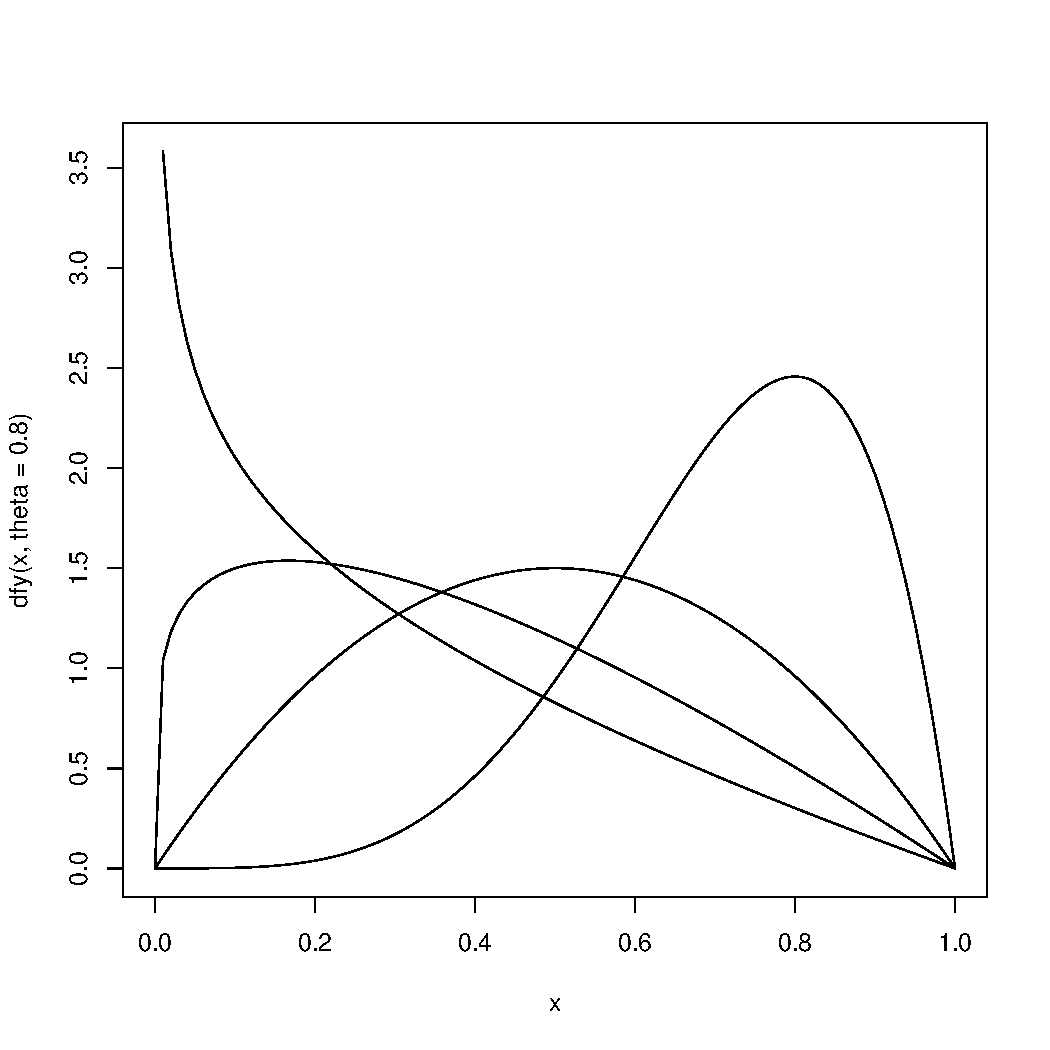
\includegraphics[width=\maxwidth]{figure/unnamed-chunk-17-1} 
\begin{kframe}\begin{alltt}
\hldef{lik} \hlkwb{<-} \hlkwa{function}\hldef{(}\hlkwc{theta}\hldef{,} \hlkwc{n}\hldef{,} \hlkwc{sly}\hldef{,}  \hlkwc{log}\hldef{=}\hlnum{FALSE}\hldef{,} \hlkwc{integra}\hldef{=}\hlnum{FALSE}\hldef{)\{}
  \hlkwa{if}\hldef{(}\hlkwd{any}\hldef{(theta}\hlopt{<}\hlnum{0}\hldef{))} \hlkwd{stop}\hldef{(}\hlsng{"valor inválido de theta"}\hldef{)}
  \hldef{res} \hlkwb{<-} \hldef{n}\hlopt{*}\hlkwd{log}\hldef{(theta)} \hlopt{+} \hldef{n}\hlopt{*}\hlkwd{log}\hldef{(theta}\hlopt{+}\hlnum{1}\hldef{)} \hlopt{+} \hldef{theta}\hlopt{*}\hldef{sly} \hlcom{# sum(log(1-y)-log(y))}
  \hlkwa{if}\hldef{(log)} \hlkwd{return}\hldef{(res)} \hlkwa{else} \hlkwd{return}\hldef{(}\hlkwd{exp}\hldef{(res))}
  \hldef{\}}


\hlkwd{curve}\hldef{(}\hlkwd{lik}\hldef{(x,} \hlkwc{n}\hldef{=}\hlnum{20}\hldef{,} \hlkwc{sly}\hldef{=}\hlopt{-}\hlnum{4.59}\hldef{),} \hlkwc{from}\hldef{=}\hlnum{3}\hldef{,} \hlkwc{to}\hldef{=}\hlnum{15}\hldef{)}
\end{alltt}
\end{kframe}
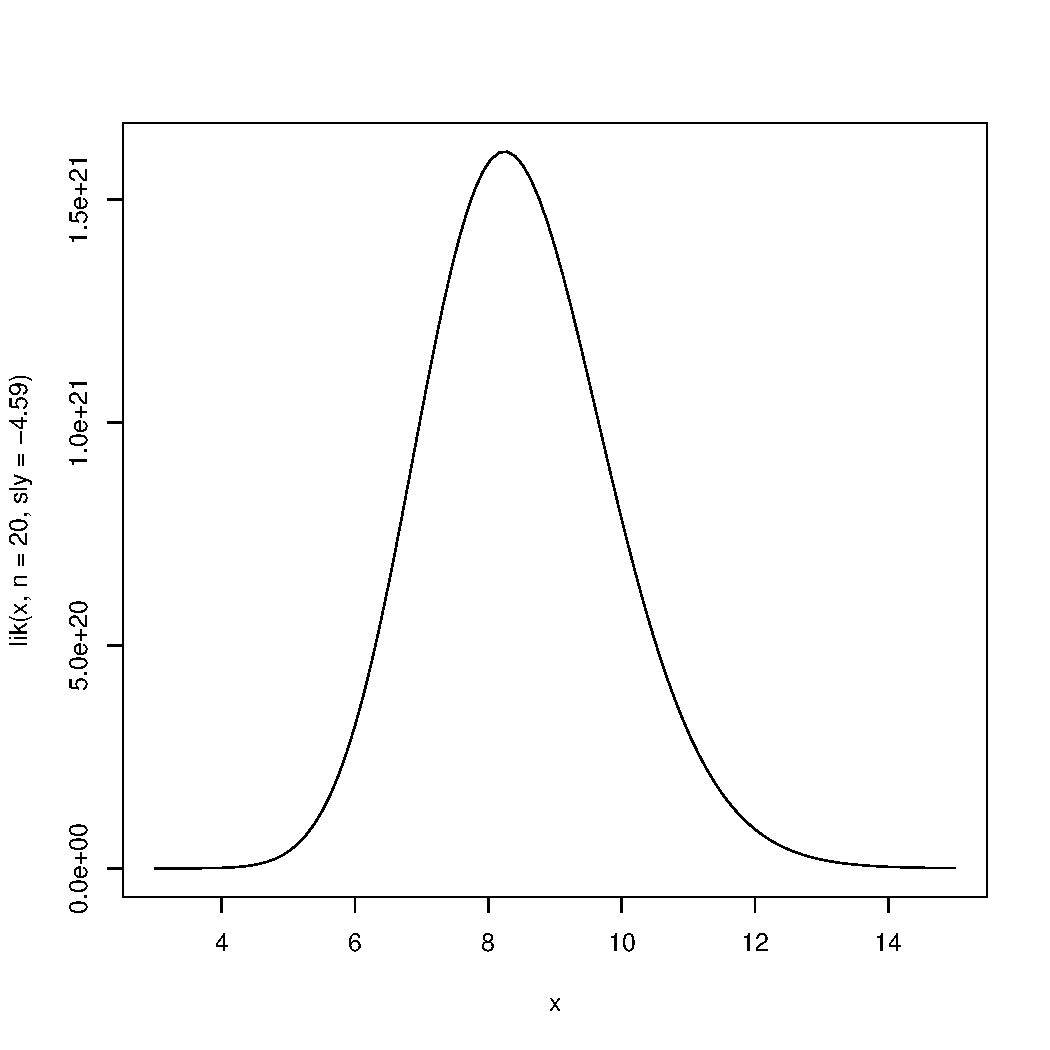
\includegraphics[width=\maxwidth]{figure/unnamed-chunk-17-2} 
\begin{kframe}\begin{alltt}
\hldef{(mle} \hlkwb{<-} \hlkwd{optimize}\hldef{(lik,} \hlkwc{interval}\hldef{=}\hlkwd{c}\hldef{(}\hlnum{0}\hldef{,} \hlnum{20}\hldef{),} \hlkwc{maximum}\hldef{=}\hlnum{TRUE}\hldef{,} \hlkwc{n}\hldef{=}\hlnum{20}\hldef{,} \hlkwc{sly}\hldef{=}\hlopt{-}\hlnum{4.59}\hldef{)}\hlopt{$}\hldef{max)}
\end{alltt}
\begin{verbatim}
## [1] 8.243
\end{verbatim}
\begin{alltt}
\hlkwd{curve}\hldef{(}\hlkwd{dfy}\hldef{(x,} \hlkwc{theta}\hldef{=mle),} \hlkwc{from}\hldef{=}\hlnum{0}\hldef{,} \hlkwc{to}\hldef{=}\hlnum{1}\hldef{)}
\end{alltt}
\end{kframe}
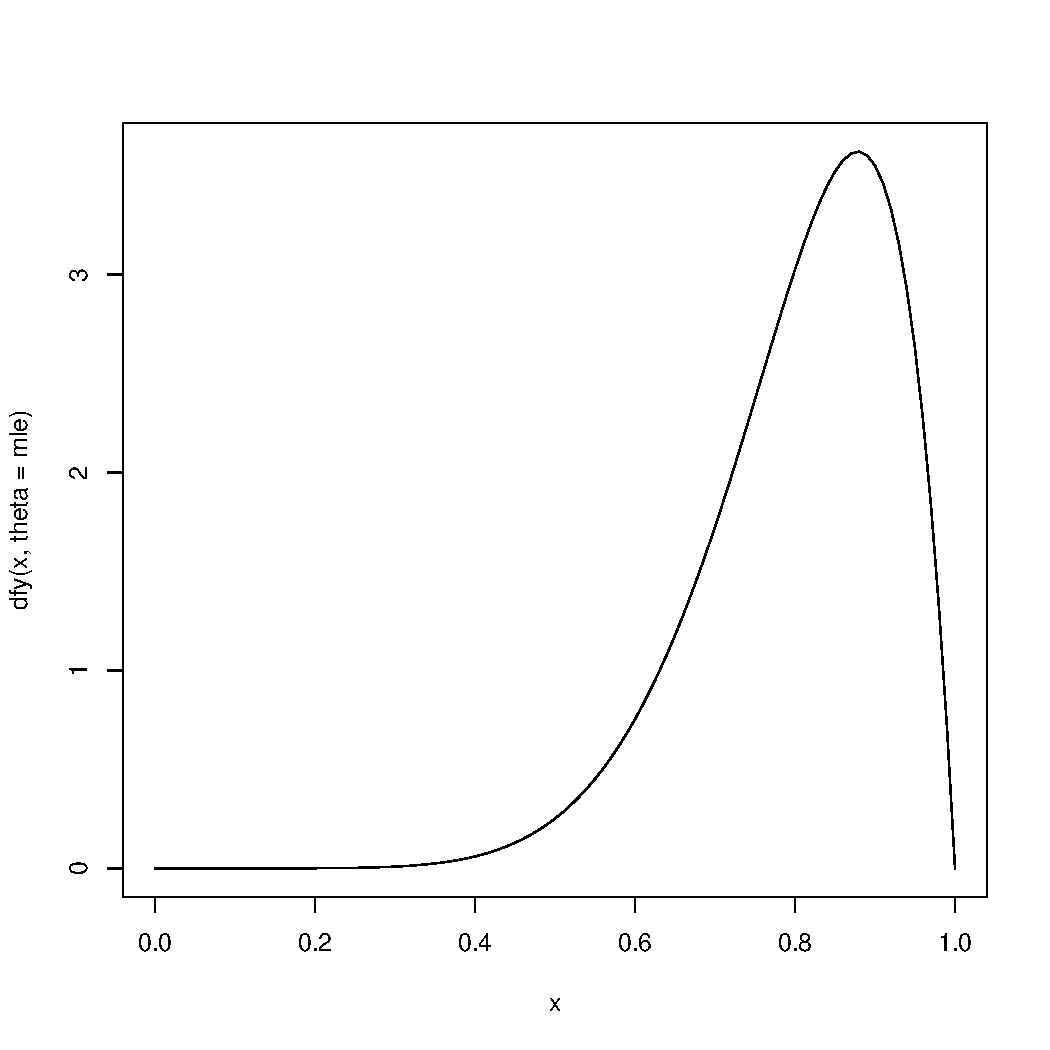
\includegraphics[width=\maxwidth]{figure/unnamed-chunk-17-3} 
\end{knitrout}
\end{solucao}

%%
%% 2018 Prova 1
%%
\item Seja $y_1, \ldots, y_n$ uma amostra aleatória de uma distribuição com função probabilidades:
\[ f(y|\theta) = \frac{{\rm e}^{-\theta}\theta^y}{y!} \; ; \;\; y=0,1,\ldots \]
e assume-se como distribuição a priori 
\[ f(\theta) = {\rm e}^{-\theta} \; ; \;\; 0 < \theta . \]
Obtenha a expressão da posteriori e da distribuição preditiva.

\begin{solucao}
  
  Obtenção da expressão da posteriori:
  \begin{align*} 
    f(y_i|\theta) &= \frac{{\rm e}^{-\theta}\theta^y_i}{y_i!} \\
    L(y|\theta) &= \frac{{\rm e}^{-n \theta}\theta^{\sum_i y_i}}{\prod_i y!} \\    
    f(\theta|y) &\propto f(\theta)  \cdot L(y|\theta) \\
                 &= {\rm e}^{-\theta} \frac{{\rm e}^{-n \theta}\theta^{\sum_i y_i}}{\prod_i y!} \\   
                 &\propto {\rm e}^{-(n+1) \theta} \theta^{\sum_i y_i}\\
              \theta|y &= {\rm Ga}(1+\sum_i y_i ; 1/(n+1))   
  \end{align*}
  Obtenção da expressão da preditiva:
  \begin{align*} 
  f(y_0|y) &= \int f(y_0|\theta, y) f(\theta|y) {\rm d}\theta = \int f(y_0|\theta) f(\theta|y) {\rm d}\theta \\
  &= \int \frac{{\rm e}^{-\theta}\theta^y_0}{y_0!} \frac{\theta^{\sum_i y_i} {\rm e}^{-(n+1)\theta}}{\Gamma(1 + \sum_i y_i) (1/(n+1)^{1 + \sum_i y_i})} {\rm d}\theta \\
  &= \frac{(n+1)^{1 + \sum_i y_i}}{y_0! \Gamma(1 + \sum_i y_i)} \int \theta^{y_0 + \sum_i y_i} {\rm e}^{-(n+2)\theta} {\rm d}\theta 
  \end{align*}
  
\begin{knitrout}
\definecolor{shadecolor}{rgb}{0.969, 0.969, 0.969}\color{fgcolor}\begin{kframe}
\begin{alltt}
\hldef{dados} \hlkwb{<-} \hlkwd{list}\hldef{(}\hlkwc{S}\hldef{=}\hlnum{32}\hldef{,} \hlkwc{n}\hldef{=}\hlnum{8}\hldef{)}

\hldef{dpred} \hlkwb{<-} \hlkwd{Vectorize}\hldef{(}\hlkwa{function}\hldef{(}\hlkwc{y}\hldef{,} \hlkwc{data}\hldef{,} \hlkwc{log}\hldef{=}\hlnum{FALSE}\hldef{)\{}
    \hldef{res} \hlkwb{<-} \hlkwd{with}\hldef{(data,} \hlopt{-}\hlkwd{lgamma}\hldef{(S}\hlopt{+}\hlnum{1}\hldef{)} \hlopt{+} \hldef{(S}\hlopt{+}\hlnum{1}\hldef{)}\hlopt{*}\hlkwd{log}\hldef{(n}\hlopt{+}\hlnum{1}\hldef{)} \hlopt{-} \hldef{(y}\hlopt{+}\hlnum{1}\hldef{)}\hlopt{*}\hlkwd{log}\hldef{(n}\hlopt{+}\hlnum{2}\hldef{))}
    \hlkwd{return}\hldef{(}\hlkwd{ifelse}\hldef{(log, res,} \hlkwd{exp}\hldef{(res)))}
    \hldef{\},} \hlsng{"y"}\hldef{)}
\hlkwd{dpred}\hldef{(}\hlnum{0}\hlopt{:}\hlnum{10}\hldef{,} \hlkwc{data}\hldef{=dados)}
\end{alltt}
\begin{verbatim}
##  [1] 1.174e-05 1.174e-06 1.174e-07 1.174e-08 1.174e-09 1.174e-10 1.174e-11 1.174e-12
##  [9] 1.174e-13 1.174e-14 1.174e-15
\end{verbatim}
\begin{alltt}
\hlkwd{plot}\hldef{(}\hlnum{0}\hlopt{:}\hlnum{100}\hldef{,} \hlkwd{sapply}\hldef{(}\hlnum{0}\hlopt{:}\hlnum{100}\hldef{, dpred,} \hlkwc{data}\hldef{=dados))}
\end{alltt}
\end{kframe}
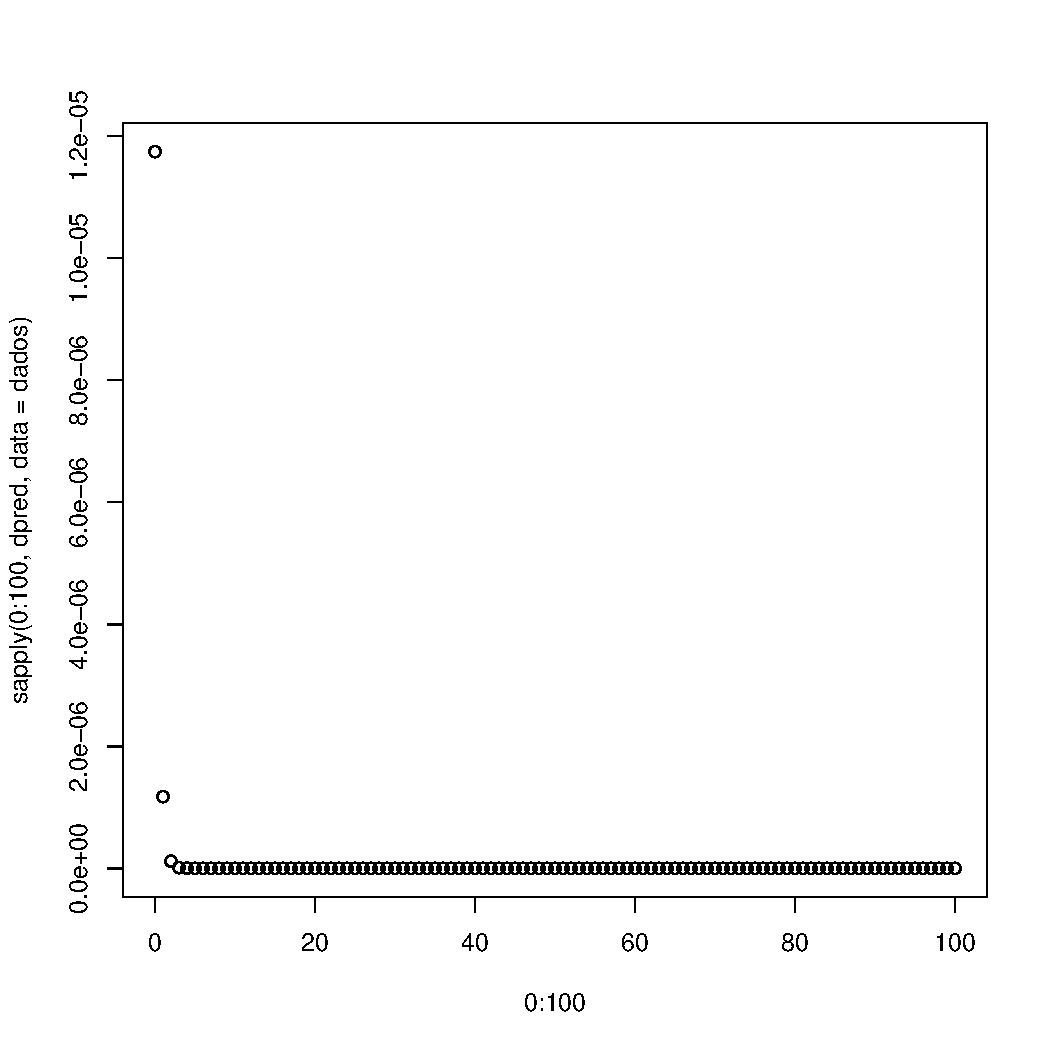
\includegraphics[width=\maxwidth]{figure/unnamed-chunk-18-1} 
\end{knitrout}
\end{solucao}

% \item Suponha que $Y$ tenha uma distribuição de Pareto ${\rm Pa}(a, b)$, em que $a$
% é conhecido mas $b$ é desconhecido. Desta forma,
% \[ f(y|b) = b a^b y^{-b-1} \; ; \;\; (y > a). \]
% Encontre a priori de Jeffreys e a correspondente distribuição posteriori para $b$ e a expressão da posteriori.
% Explique como poderiam ser obtidos resumos (média, mediana, quantis, intervalos) da distribuição posteriori neste caso.

\item A distribuição de falhas ao longo do comprimento de uma fibra artificial segue um processo de Poisson, 
  de modo que o número de falhas de um comprimento $l$ da fibra é ${\rm Po}(l\theta)$. 
  Pouco se sabe sobre $\theta$. 
  O número de falhas obtidos em 5 de fibras de comprimentos de 10, 15, 25, 30 e 40 metros, respectivamente, foram de 3, 2, 7, 6 e 10. 
  Encontre a distribuição preditiva para o número de falhas em outra fibra com 60 metros de comprimento.
  Explique os passos que seriam executados para obter amostras e resumos da preditiva por simulação estocástica.

\begin{solucao}
  % \begin{align*} 
  A distribuição de probabilidade para a variável observável $Y$ é:
  \[    f(y_i|\theta) = \frac{{\rm e}^{-L_i \theta}(L_i \theta)^y_i}{y_i!} \]
  % \end{align*}
  A priori conjugada neste caso é uma distribuição Gama.
  \[ f(\theta|p, q) = \frac{q^p}{\Gamma(p)} \theta^{p-1} {\rm e}^{-q \theta} \] 
  Obtenção da expressão da posteriori:
  \begin{align*} 
    L(y|\theta) &= \frac{{\rm e}^{-\theta \sum_i L_i } \prod_i (N_i^{y_i}) \theta^{\sum_i y_i}}{\prod_i y!} \\    
    f(\theta|y) &\propto f(\theta)  \cdot L(y|\theta) \\
                &\propto \theta^{p+(\sum_i y_i) -1} {\rm e}^{- (q+\sum_i L_i)\theta} \\   
    \theta|y &\sim {\rm Ga}(p+\sum_i y_i ; q+\sum_i L_i )   
  \end{align*}
  Obtenção da expressão da preditiva:
  % \begin{align*} 
  %   f(y_0|y) &= \int f(y_0|\theta, y) f(\theta|y) {\rm d}\theta \stackrel{ind. cond.}{=} \int f(y_0|\theta) f(\theta|y) {\rm d}\theta \\
  %                &= \int  \frac{{\rm e}^{-L_0 \theta}(L_0 \theta)^y_i}{y_0!} \frac{\theta^{\sum_i y_i} {\rm e}^{-(n+1)\theta}}{\Gamma(1 + \sum_i y_i) (1/(n+1)%^{1 + \sum_i y_i})} {\rm d}\theta \\
  %                &= \frac{(n+1)^{1 + \sum_i y_i}}{y_0! \Gamma(1 + \sum_i y_i)} \int \theta^{y_0 + \sum_i y_i} {\rm e}^{-(n+2)\theta} {\rm d}\theta 
  %              \end{align*}
\end{solucao}   

%% 
%% 2018 Prova 2
%% 

\item O número de defeitos em um rolo de 1200 metros de uma fita magnética possui distribuição 
  Poisson($\theta$). A distribuição priori para $\theta$ é Gama($3;1$). 
  Quando cinco rolos deste tipo são selecionados ao acaso, o número de defeitos encontrados em cada um deles é: 2, 2, 6, 0 e 3, respectivamente. 
  Determine a distribuição a posteriori de $\theta$.
  
% \item Seja $y_1, \ldots, y_n$ uma amostra aleatória de uma distribuição com função probabilidades:
%   \[ f(y|\theta) = \theta \exp\{-\theta y\} \]
%   Obtenha a priori de Jeffreys, 
%   a expressão da posteriori e da distribuição preditiva.
  
\item Considere o problema de uma regressão linear simples usual com o regressor $x$ e a variável resposta $Y$.
  Deseja-se implementar um algorítmo para análise bayesiana deste modelo.
  Descreva os passos que seriam necessários e
  obtenha as expressões relevantes para implementação do algorítmo. 
  Inclua no algoritmo a possibilidade de predição.
  Faça escolhas qdo necessário como, por exemplo, de priori.
  
%% 
%% 2018 Prova 3
%% 

  
\item Foi visto no curso e em provas anteriores que para o modelo (verossimilhança) Poisson
  a priori conjugada é uma distribuição Gama.
  Entretanto pode-se pensar em outras prioris tal como uma log-normal, 
  ou seja, um modelo com $Y \sim {\rm P}(\lambda)$ e $\log(\lambda) \sim {\rm N}(a, b)$.
  É possível obter uma posteriori em forma fechada e conhecida neste caso?
  Qual a expressão da posteriori (se necessário a uma constante de proporcionalidade).
  Se voce tivesse dados de contagem para analisar sob o paradigma Bayesiano com este modelo,
  como procederia? Qual ou quais procedimentos adotaria para obter inferências à posteriori?
  
\item Encontre a priori de Jeffreys para $\theta$ no modelo geométrico:
  \[ f(x|\theta) = (1-\theta)^{x-1} \theta \; ; \;\; x=1, 2, \ldots  \]
  para uma amostra $x_1, \ldots, x_n$.
  Obtenha as expressões da posteriori e da preditiva.\\
  Considere uma amostra de dados: $5, 4, 7, 3, 2, 5, 6, 8, 10$
  Forneça a expressão da posteriori e o um valor predito para uma nova observação.

\item Considere o problema de uma regressão linear simples usual com o regressor $x$ e a variável resposta $Y$.
Deseja-se implementar um algorítmo para análise bayesiana deste modelo.
Descreva os passos que seriam necessários e
obtenha as expressões relevantes para implementação do algorítmo. 
Inclua no algoritmo a possibilidade de predição.
Faça escolhas qdo necessário como, por exemplo, de priori.

% \item Escreva de maneira suscinta (um parágrafo com no máximo 10 linhas) como voce explicaria para um 
%   pesquisador de outra área as características da análise bayesiana em contraste com outra(s) abordagem(ens).

\item A classificação de qualidade de um componente elétrico é excelente ($y = 1$), bom ($y = 2$) ou ruim ($y = 3$). A probabilidade de vários níveis de qualidade dependem da fábrica onde é produzido ($\theta_1 = 0$: fábrica A, $\theta_1 = 1$: fábrica B) e do tipo de máquina ($\theta_2 = 0$: máquina I, $\theta_2 = 1$: máquina II, $\theta_2 = 2$: máquina III). As probabilidades para $y = 2$ são dadas pela Tabela~\ref{tab:exerc1a-cap4}.
Além disso, distribuição conjunta de $(\theta_1, \theta_2)$ é dada na Tabela~\ref{tab:exerc1b-cap4}.
Encontre a distribuição posteriori conjunta de $\theta_1, \theta_2|y = 2$ e cada uma das distribuições marginais. Tendo observado $y = 2$:
\begin{enumerate}
\item Qual a combinação fábrica/máquina é a mais provável de ter produzido esse componente?
\item Qual a distribuição posteriori (conjunta)?
\item Quais são as distribuições marginais?
\item E as condicionais?  
\item Esboce gráficos para os itens anteriores
\end{enumerate}

%%
%% 2025 prova 2
%%

\item Seja $Y$ uma variável aleatória com distribuição normal de média igual a zero
  e precisão $\tau$ sendo $\tau = 1/\sigma^2$. Será tomada uma amostra de $n$ observações
  $y_1, y_2, \ldots y_n$ deste modelo.
  \begin{enumerate}
  \item Qual a priori conjugada para $\tau$?
  \item Qual é a distribuição posteriori para a priori do item anterior?
  \item Qual a priori de Jeffreys $\tau$?
  \item Qual é a distribuição posteriori para a priori de Jeffreys?
  \end{enumerate}

\begin{solucao}
\paragraph{\bf Solução} \mbox{} \\
  \begin{itemize}
  \item Priori conjugada: $\tau \sim {\rm Gama}(a, b):$ 
    \[
      \pi(\tau) \propto \tau^{a-1} e^{-b\tau}.
    \]
    
  \item Posteriori para priori conjugada
    \[
      \tau|y \sim \mathrm{Gama}\left(a + \frac{n}{2},\; b + \frac{1}{2} \sum_{i=1}^n y_i^2\right).
    \]
  \item Priori de Jeffreys
    \[
      \pi_J(\tau) \propto 1/\tau.
    \]
  \item Posteriori para priori de Jeffreys
    \[
      \pi(\tau|y) \propto \tau^{n/2 - 1} \exp\left(-\frac{\tau}{2} \sum y_i^2\right).
    \]
  \end{itemize}
\end{solucao}





\item Seja uma variável aleatória $Y$ e o seguinte modelo de probabilidades: $Y|\theta \sim {\rm Bin}(n, \theta)$.
  Adota-se como priori de $\theta$ uma mistura das distribuições ${\rm Beta}(2, 10)$ e $ {\rm Beta}(4, 2)$ com pesos 0,20 e 0,80, respectivamente.
  Uma amostra forneceu $y = 6, n = 20$. Esboce os gráficos de cada componentes da priori. Obtenha a expressão da posteriori e um esboço do seu gráfico.

\begin{solucao}
\paragraph{\bf Solução} \mbox{} \\
  Priori:
  \[ P(\theta) = 0.20 * Beta(2,10) + 0.80 * Beta(4,2).\]
  Observou-se \(y=6, n=20\). Verossimilhança:
  \[ L(\theta|y) \propto \theta^6 (1-theta)^{20-6}. \]
  Posteriori:
  \[ P(\theta) = 0.4159 * Beta(8,24) + 0.5841 * Beta(10,16).\]

\end{solucao}
  





\begin{table}[ht!]
\centering
\caption{Probabilidades condicionais $y = 2$}
\label{tab:exerc1a-cap4}
  \begin{tabular}{c| c c}
    Pr($y = 2|\theta_1, \theta_2$)         &$\theta_1 = 0$          &$\theta_1 =1$\\
    \hline
    $\theta_2 = 0$                         &0,3                    &0,2\\
    $\theta_2 = 1$                         &0,4                    &0,2\\
    $\theta_2 = 2$                         &0,6                    &0,3\\
    \hline
  \end{tabular}
\end{table}

\begin{table}[ht!]
\centering
\caption{Probabilidade a priori das combinações fábrica/máquina}
\label{tab:exerc1b-cap4}
  \begin{tabular}{c| c c}
    Pr($\theta_1, \theta_2$)               &$\theta_1 = 0$          &$\theta_1 =1$\\
    \hline
    $\theta_2 = 0$                         &0,1                    &0,2\\
    $\theta_2 = 1$                         &0,2                    &0,3\\
    $\theta_2 = 2$                         &0,1                    &0,1\\
    \hline  
\end{tabular}
\end{table}

%\begin{extra}
%{\it Obtenha gráficos da priori, verossimilhança e posteriori deste problema.}
%\end{extra}


\item Explique os tópicos a seguir, incluindo exemplos, tendo como referência as aulas e materiais do curso.
\begin{enumerate}
  \item Priori imprópria.
  \item Princípio da verossimilhança.
  \item Reparametrizações, prioris equivalentes e invariância.
\end{enumerate}

  
\item Seja $Y \sim {\rm Gamma}(\alpha, \lambda)$ com priori (independente) $\alpha \sim {\rm Gama}(a, b)$ e $\lambda \sim {\rm Gamma}(c, d)$
  em que $\lambda, b \; {\rm e }\; d$ são parâmetros de taxa.

  \begin{enumerate}
  \item Obtenha a expressão da posteriori $f(\alpha, \lambda|y)$.
  \item Obtenha a expressão da posteriori $f(\lambda|\alpha, y)$.
  \item Obtenha a expressão da posteriori $f(\alpha|\lambda, y)$.
  \item Obtenha a expressão da posteriori $f(\lambda|y)$.
  \item Obtenha a expressão da posteriori $f(\alpha|y)$.
  \item Explique como obter simulações de cada uma das distribuições acima. 
  \item Explique como obter simulações da marginal (preditiva a priori). 
  \item Explique como obter simulações da marginal (preditiva a posteriori). 
  \item Foi proposto o seguinte algorítmo para simular da posteriori conjunta:
    \begin{enumerate}
    \item Escolha um valor inicial para $\alpha$.
    \item Simule um valor de $f(\lambda|\alpha, y)$, em que $\alpha$ é o último valor obtido.
    \item Simule um valor de $f(\alpha|\lambda, y)$, em que $\lambda$ é o último valor obtido.
    \item Repita os dois passos anteriores $N$ vezes.     
    \item Os $N$ pares $\alpha, \lambda$ são uma amostra de $f(\alpha, \lambda|y)$.
    \end{enumerate}
  \end{enumerate}

\begin{solucao}
\paragraph{\bf Solução} \mbox{} \\ 
\begin{itemize}
\item Conjunta
\item Condicionais
\item Marginais
\end{itemize}
\end{solucao} 





\item  Um teste para detectar a presença ou não de certa doença é aplicado em uma população. Sabe-se que o teste acerta 90\% dos que possuem a doença ({\it sensibilidade}) e 80\% dos que não a possuem ({\it especificidade}). A ocorrência da doença na população alvo é de 2\% ({\it prevalência}).
O interesse é realizar uma análise bayesiana completa. Pede-se, explicando passo a passo:
\begin{enumerate}
\item {\bf Análise da Posteriori:} Determinar a probabilidade de um indivíduo ter a doença, dado um resultado positivo ({\it valor preditivo positivo}), e a probabilidade de não ter a doença, dado um resultado negativo ({\it valor preditivo negativo}).
\item {\bf Análise pelo Fator de Bayes:} Avaliar a força da evidência fornecida por um teste positivo em favor da hipótese de que o paciente tem a doença, em comparação com a hipótese de que não a tem.
\item {\bf Análise pela Teoria da Decisão:} Suponha que a perda (ou custo) de um diagnóstico {\it falso negativo} (diagnosticar "não doente" quando a pessoa tem a doença) seja 5 vezes maior que a perda de um diagnóstico {\it falso positivo} (diagnosticar "doente" quando a pessoa não tem a doença). Qual seria a decisão ótima entre diagnosticar como 'Doente' ou 'Não Doente' para cada resultado do teste, a fim de minimizar a perda esperada?
\item Discuta os resultados.
\item Discuta as características de cada e as diferenças dos métodos.
\end{enumerate}

\item Considere o contexto predição (a posteriori) Bayesiana, porém deseja-se obter somente o vaslor esperado e a variância da preditiva. Obtenha as expressões destas quantidades no modelo
  de verossimilhança Poisson com priori Gamma.

\item Explique de forma concisa a diferença entre intervalos frequentista, de verossimilhança e
  bayesiano (de quantis os HDI)


\item Descreva o modelo sendo ajustado, distribuições envolvidas, parâmetros e constantes.
  Esboce ainda a estrutura dos dados nas seguintes declarações de modelos em JAGS.

\begin{enumerate}

  \item
\begin{verbatim}
model{
  for (i in 1:N){
    x[i] ~ dbern(p)
  }
  p ~ dbeta(alpha, beta)
  alpha <- 1
  beta <- 1
}
\end{verbatim}

  \item
\begin{verbatim}
model {
  for (i in 1:n) {
    y[i] ~ dnorm(0, tau)
  }
  tau ~ dgamma(a, b) 
  sigma <- 1 / sqrt(tau)
}
\end{verbatim}

\item
\begin{verbatim}
model{
  for(i in 1:M){
     for(j in 1:N){
        y[i,j] ~ dnorm(mu[i], tau)
     }
     mu[i] ~ dnorm(theta, tauD)
  }
  tau <- pow(sigma, -2)
  sigma ~ dunif(0, 100)
  theta ~ dnorm(0, .001)
  tauD <- pow(delta, -2)
  delta ~ dunif(0, 100)
}
\end{verbatim}

\item
\begin{verbatim}
model {
    for (i in 1:n) {
        y[i] ~ dgamma(alpha, lambda)
    }
  alpha ~ dgamma(a, b)
  lambda ~ dgamma(c, d)
}

\end{verbatim}

\item
\begin{verbatim}
model {
  y ~ dbin(theta, n)
  k ~ dcat(p)
  theta ~ dbeta(alpha[k], beta[k])
}
\end{verbatim}

\item
\begin{verbatim}
model{
for(i in 1:n){
    y[i] ~ dpois(mu[i])
    mu[i] <- ifelse(i > k, lambda, theta)
}
k ~ dcat(ano[])
theta ~ dgamma(a1, b1)
lambda ~ dgamma(a2, b2)
dif <- lambda - theta
ib1 ~ dgamma(c1, d1)
b1 <- 1/ib1
ib2 ~ dgamma(c2, d2)
b2 <- 1/ib2
a1 <- 0.5
a2 <- 0.5
c1 <- 0.1
c2 <- 0.1
d1 <- 1
d2 <- 1
}
\end{verbatim}
\end{enumerate}



\end{enumerate}

\end{document}

